\documentclass[english, msc, oneside]{layout/observatory-thesis}
\usepackage[utf8]{inputenx}



\usepackage{graphicx} 
\usepackage{amsmath,amssymb,amsthm}

\usepackage{multicol}
\usepackage{subcaption}
\usepackage{caption}

\usepackage{pdfpages}
\usepackage{mdframed}
\usepackage{lipsum}

\usepackage{fancyhdr}
\usepackage{ragged2e}
\usepackage{amsfonts} 
\usepackage{setspace}           
\usepackage{float}

\theoremstyle{definition}
\newtheorem{exmp}{Example}[section]
\newtheorem{theorem}{Theorem}[section]
\newtheorem{corollary}{Corollary}[theorem]
\newtheorem{lemma}[theorem]{Lemma}

\newmdtheoremenv{theo}{\textbf{Results}}


\begin{document}


\title{\textbf{A Survey to Infer on the \\Effects of COVID-19}}
\subtitle{Exploring the Ripple Effects of the Pandemic on Daily Habits, Social Interactions, and Well-being} 
\subject{\thesistypeshort Project Report}
\author{M.Tech CrS $1^{st}$ Semester Students}
\supervisor{Prof. ARGHA SARDAR}
\projectstart{October 2023}
\projectend{December 2023}
\affiliation{M.Tech. First Year, ISI Kolkata}
\address{Indian Statistical Institute, Kolkata 700108, India}
\coverimage{layout/figures/free_frontpage/2.jpg}


\frontmatter 

\makecover 
\maketitle 

\disclaimer

\chapter{Abstract}

\

The new coronavirus $SARS-CoV-2$ that triggered the COVID-19 pandemic arose as an unprecedented worldwide health disaster that drastically altered life as we know it. This contagious disease has spread quickly across continents since it was first discovered in late 2019, posing a threat to global healthcare systems, economy, and social norms.

\

In addition to posing serious risks to public health, this epidemic has caused significant socioeconomic upheavals that have changed the course of our everyday lives. It is now critical to understand the complexities of this viral outbreak, the ways in which it spreads, the effects it has on different populations, and how to establish effective mitigation techniques.

\

In this project, we delve into a comprehensive analysis of the multifaceted dimensions of the COVID-19 pandemic. We explore the emergence of vaccines and treatments, worldwide response initiatives, clinical manifestations, epidemiology, transmission dynamics, and societal implications. Understanding these aspects is crucial not only for navigating the crisis but also for preparing and fortifying ourselves against potential future pandemics.

\

This study attempts to provide light on the intricate interactions between the virus and society by carefully examining scientific studies, statistical data, and socio-economic analysis. Through acquiring a profound understanding of the effects of COVID-19, we hope to add to the current conversation, promoting well-informed choices and supporting initiatives to address this worldwide threat.

\

Our analysis is based on the data collected from 230 individuals. 
\tableofcontents

\mainmatter 

\chapter{The Survey}
\section{DATA DESCRIPTION}

In order to ensure the success of our work, we formulate a set of questions and obtain the necessary data using a Google Form. To access the form, please visit: \url{https://forms.gle/VDTpe4S4yUoHkkbG6}

\section*{Personal Information}
\begin{enumerate}
    \item \textit{Name:}
    \item \textit{Age:}
    \item \textit{Gender:}
    \item \textit{Current Employment Status:}
    \item \textit{Profession:}
\end{enumerate}

\section*{Family and Vaccination Status}
\begin{enumerate}[resume]
    \item Number of Heads in Family (Including yourself):
    \item Have you been vaccinated completely against COVID-19?
\end{enumerate}

\section*{Occupational and Activity Engagement}
\begin{enumerate}[resume]
    \item Were you engaged in any occupation / project / institutional activities during specific times?
    \item Were you engaged in those activities mostly from home during specific times?
\end{enumerate}

\section*{Outdoor Activities and Testing}
\begin{enumerate}[resume]
    \item How often did you go outside at the time of Corona?
    \item Had you tested yourself for COVID-19?
    \item Were the results positive?
\end{enumerate}

\section*{Health and Chronic Conditions}
\begin{enumerate}[resume]
    \item Rate the severity of COVID-19 infection on your health ?
    \item Did you have any chronic disease / co-morbidity before COVID-19?
    \item Please rate the change in severity of the chronic disease before and after the pandemic on a scale of $0$ to $5$ (With $0$ being Did Not Change / Not Applicable and $5$ being Reached a Critical Level.)
\end{enumerate}

\section*{Mental Health and Physical Well-being}
\begin{enumerate}[resume]
    \item Have you faced any unusual mental health issues during COVID-19?
    \item Please mention an approximate value for the following quantity (in Kg): Your weight after the pandemic - Your weight before the pandemic (Subtract, negative values may arise.)
\end{enumerate}

\section*{Financial and Medical Impact}
\begin{enumerate}[resume]
    \item Were any of your family members tested positive for COVID-19?
    \item Were there any deaths due to COVID-19 in your family?
    \item Please mention an approximate value for the following quantity (in \textit{INR}): Monthly medical expenses of your family after the pandemic - That before the pandemic (Subtract, negative values may arise.)
\end{enumerate}

\section*{Hygiene Practices and Adherence}
\begin{enumerate}[resume]
    \item Have you used the following items? (\textit{Before/During/After} COVID-19)
    \begin{itemize}
        \item \textit{Sanitizer.}
        \item \textit{Face mask.}
        \item \textit{Head mask.}
        \item \textit{Hand gloves.}
        \item \textit{Face shield.}
    \end{itemize}
    \item Have you followed the mentioned rules/practices?
    \begin{itemize}
        \item \textit{Safe distancing.}
        \item \textit{No touch product acceptance.}
        \item \textit{Washing marketed products thoroughly.}
        \item \textit{Washing hands with soap for a minimum of $20$ sec.}
        \item \textit{Physically exercising.}
    \end{itemize}
\end{enumerate}

\section*{Lifestyle Changes}
\begin{enumerate}[resume]
    \item How much have you depended on the cooked-food delivery system? (Choose the closest answers.)
    \item How have your average screen times (on phone, TV, etc.) been? (Choose the closest answers.)
    \item Considering its severity, if there is another epidemic like COVID-19 within the next $20$ years, do you have any hygiene plans to combat it?
\end{enumerate}

\section*{Perception and Future Preparedness}
\begin{enumerate}[resume]
    \item What has been COVID-19's effect on the growth of education in your family?
    \item Do you have economic backup plans for any upcoming epidemic within the next $20$ years?
    \item How have the following aspects changed in your life after COVID-19?
    \begin{itemize}
        \item \textit{Social interaction.}
        \item \textit{Annual family income.}
        \item \textit{Monthly family expenses.}
        \item \textit{Screen-time.}
        \item \textit{Dependence on the ready-made delivery system.}
    \end{itemize}
    \item Considering the general reluctance to adapt to the new lifestyle during the COVID-19 pandemic, how likely are you to start following the safety rules imposed (by the nationally accepted medical societies), if there is a pandemic in the next $20$ years?
    \item Is there any other experience/changes in your life due to the pandemic that you would wish to share with us? If '\textit{Yes}', please write.
\end{enumerate}

\chapter{Demographic Details}
\section{Male-Female Ratio}

The survey aimed to capture a diverse range of experiences related to the effects of COVID-19 on lifestyle changes. One significant aspect of this diversity is the representation of different genders among the respondents.

\begin{figure}[h!]
	\centering
	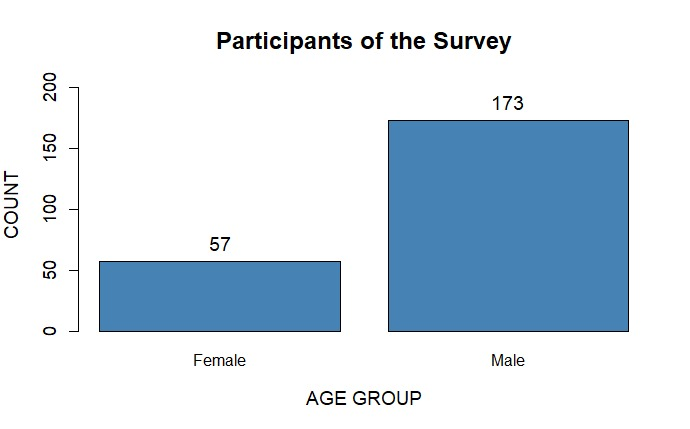
\includegraphics[width=0.7\linewidth]{IMAGES/Image 1.jpg}
	\caption{Male-Female Ratio}
	\label{G1}
\end{figure}

\

Figure \ref{G1} presents the results of a survey with $230$ participants corresponding to their genders. The figure is a Bar plot clearly representing $57$ female and $173$ male participants who took part in the survey.

\ 

\section{Employment Status}

\begin{figure}[h!]
	\centering
	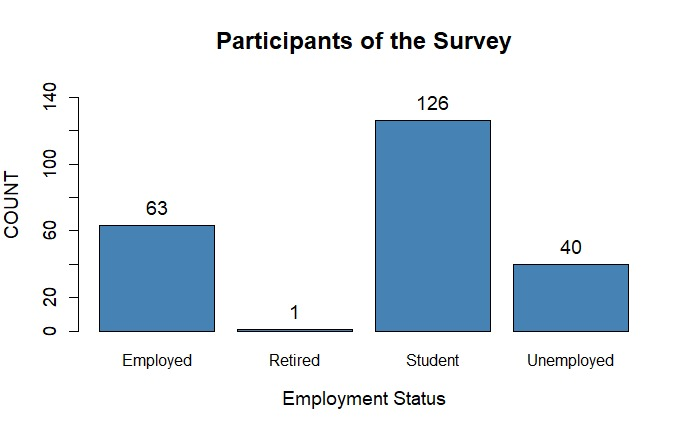
\includegraphics[width=0.75\linewidth]{IMAGES/Image 2.jpg}
	\caption{Employment Status}
	\label{G2}
\end{figure}

\ 

Figure \ref{G2} presents the results of the above-mentioned survey categorized by the
employment status of the participants. The employment status of the participants shows
that $63$ are employed, $1$ is retired, $126$ are students and $40$ are unemployed.

\ 

The survey indicates that the majority of participants are students, with a significant number
of employed and unemployed individuals and a very small representation of retired persons.
The data highlights the distribution of\\ employment status among the survey participants
and provides insights into the demographic composition of the sample.

\ 

\section{Heads in Family}

\begin{figure}[h!]
	\centering
	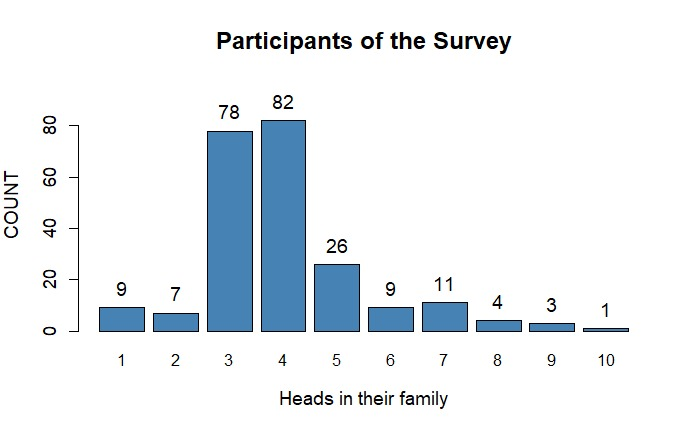
\includegraphics[width=0.75\linewidth]{IMAGES/Image 3.jpg}
	\caption{Heads in Family}
	\label{G3}
\end{figure}

\ 

In Figure \ref{G3} the document provides an overview of our survey with respect to the number of heads in the families of the participants.

\

The data indicates that the majority of participants had $3$ to $5$ members in their families,
with a few outliers having $1, 2, 6, 7, 8, 9,$ or $10$. Overall, the survey aimed to gather
information about family size within the specified sample observations.

\section{Age Group}

\begin{figure}[h!]
	\centering
	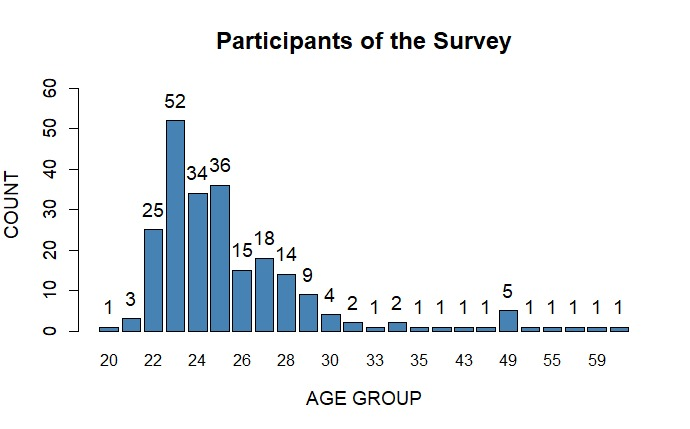
\includegraphics[width=0.8\linewidth]{IMAGES/Image 4.jpg}
	\caption{Age Group}
	\label{G4}
\end{figure}

\ 

The data represented in Figure \ref{G4} indicates the number of participants corresponding to their ages.

\ 

The data, shows that the majority of the participants, who took part in the survey, are aged between $20$ and $30$ with $52$, $34$ and $36$ persons of age $23$, $24$ and $25$ respectively. Ages of more than $34$ have been rare, although we had $5$ occurrences of age $49$ as an exception. This plot signifies that our sample data greatly consists observations of people having age between $20$ and $30$.

\chapter{Data Analysis}
\section{Families getting effected}

\begin{figure}[h!]
	\centering
	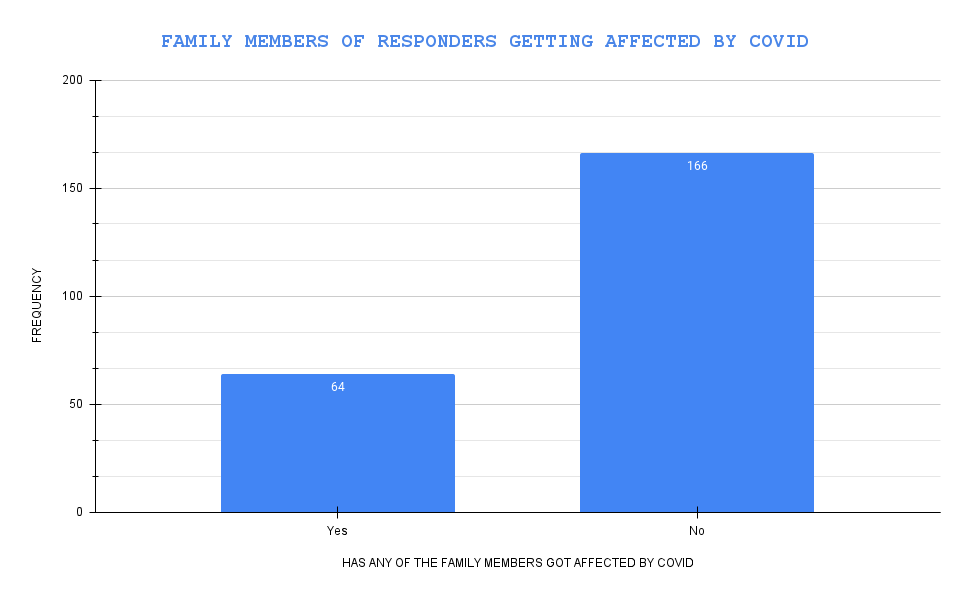
\includegraphics[width=0.5\linewidth]{IMAGES/Image 26.png}
	\caption{Effected by COVID in Family}
	\label{G26}
\end{figure}

Figure \ref{G26} represents that $64$ participants have reported having family members have been affected by COVID-19, while the remaining $166$ participants indicated that none of their family members had been impacted by the virus.


\subsection{Deaths}
\begin{figure}[h!]
	\centering
	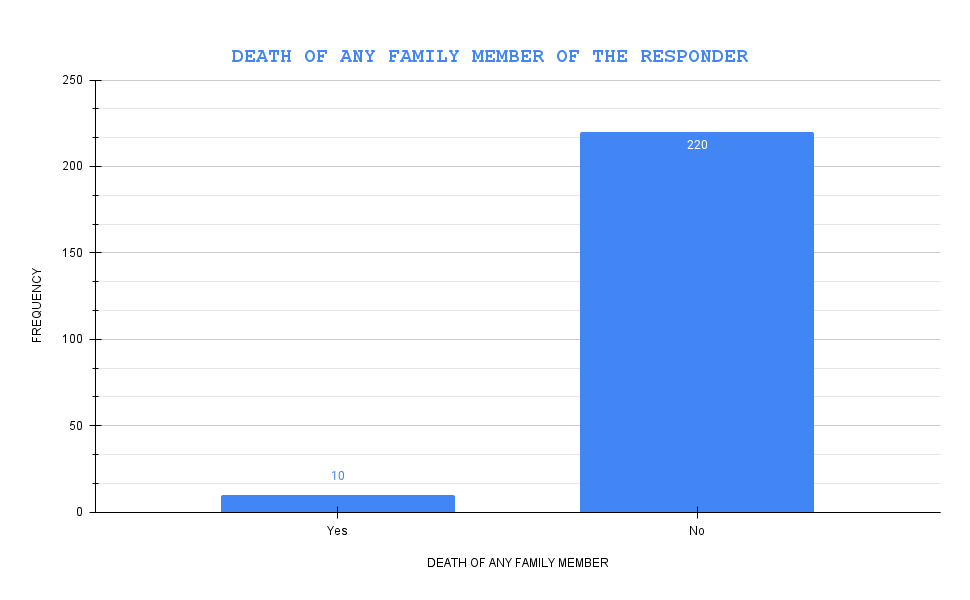
\includegraphics[width=0.5\linewidth]{IMAGES/Image 27.png}
	\caption{Deaths due to COVID in Family}
	\label{G27}
\end{figure}

In Figure \ref{G27}, it is observed that among the $230$ participants, $10$ individuals have encountered the loss of a family member due to COVID.

\newpage

\section{Family Income and Expenses}

\subsection{Annual family Income}

\begin{figure}[h!]
	\centering
	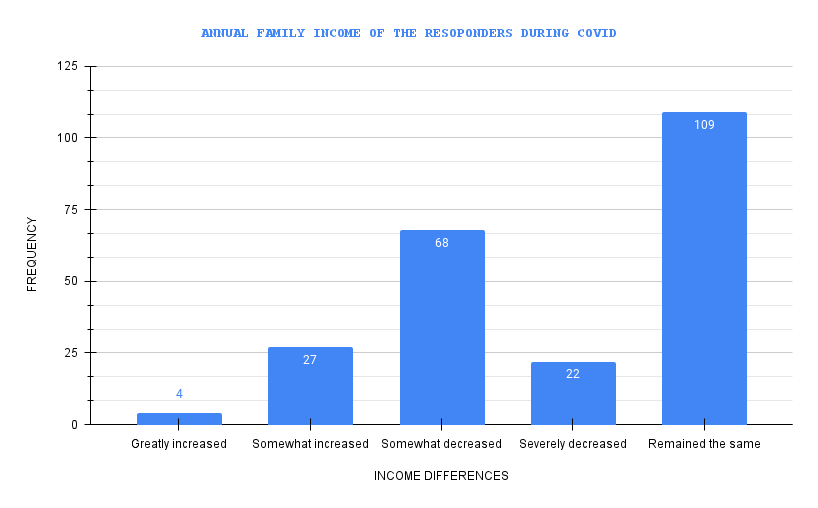
\includegraphics[width=0.6\linewidth]{IMAGES/Image 19.png}
	\caption{Income and Expenses}
	\label{G19}
\end{figure}

 Figure \ref{G19} indicates the fluctuations in annual family income among respondents during the COVID-19 pandemic. The majority, of $109$ participants have reported no significant change in their family income. However, $68$ participants experienced a bit decrease, while $22$ participants faced a substantial decrease. On a positive note, $27$ participants saw a moderate increase, and $4$ participants reported a significant boost in their annual family income.

\subsection{Annual family Expenses}

\begin{figure}[h!]
	\centering
	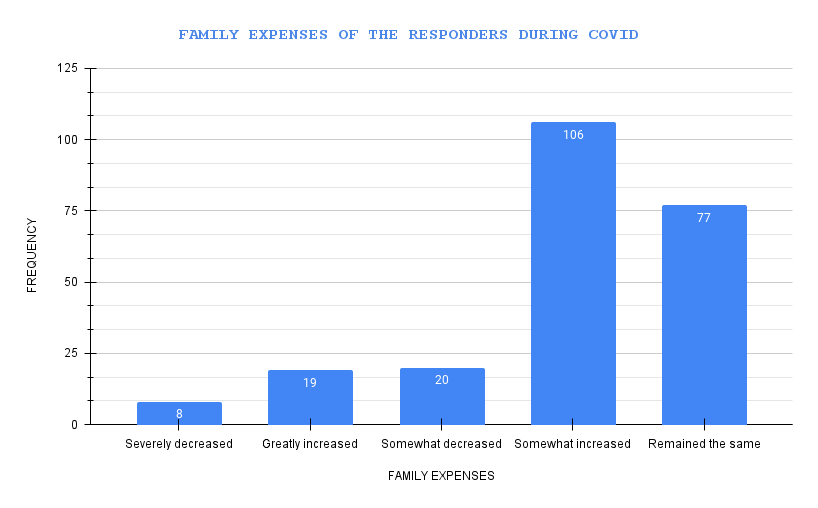
\includegraphics[width=0.6\linewidth]{IMAGES/Image 20.png}
	\caption{Income and Expenses}
	\label{G20}
\end{figure}
 
However, for the majority of participants, monthly family expenses have either remained constant or experienced a slight increase. Figure \ref{G20} shows that for $106$ participants, the monthly expenses have somewhat increased, while for $77$ participants, family expenditures have stayed the same.

\newpage

\subsection{Comparative Analysis of Family Expenditure Across Different\\ Employment Categories}

\begin{figure}[h!]
	\centering
	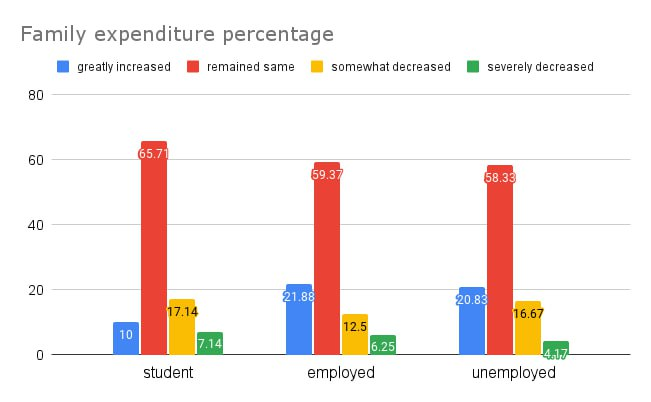
\includegraphics[width=0.9\linewidth]{IMAGES/Image 33.jpeg}
	\caption{Percentage of Family Expenditure}
	\label{G33}
\end{figure}
$$\textit{Student($126$) | Employed($63$) | Unemployed($40$)}$$

\ 

The bar chart depicts the distribution of family expenditure levels across three distinct categories of individuals: \textit{students, employed individuals, and the unemployed}. Expenditure levels are classified into four groups: "\textbf{Greatly Increased}," "\textbf{Remained Same}," "\textbf{Somewhat Decreased}," and "\textbf{Severely Decreased.}"

\ 

Let’s analyze the Family Expenditure, So for students, $10\%$ experienced a substantial increase in family expenditure, while a majority $(65.71\%)$ maintained a consistent level. Approximately $17.14\%$ observed a moderate decrease, and a smaller portion $(7.14\%)$ faced a significant reduction.

\

Among employed individuals, $21.88\%$ noted a substantial rise in family expenditure, while the largest portion $(59.37\%)$ sustained a steady spending pattern. About $12.5\%$ experienced a moderate decline, and a smaller proportion $(6.25\%)$ encountered a considerable drop.

\

Unemployed individuals experienced noteworthy changes as well, with $20.83\%$ noting a significant increase, $58.33\%$ maintaining consistency, $16.67\%$ observing a moderate reduction, and a minority $(4.17\%)$ facing a substantial decrease in family spending.

\newpage 

\

\textbf{Key Insights : }

\ 

Consistency Among Employees:  The largest percentage of both employed individuals and students maintained similar family expenditure levels, with around $59.37\%$ and $65.71\%$, respectively, staying consistent.

\ 

Impact of Unemployment: Unemployed individuals showcased a slightly higher percentage in experiencing increased family expenditure $(20.83\%)$ compared to employed individuals $(21.88\%)$.

\ 

Variance in Decreased Expenditure: There is a notable difference in the percentage of individuals who experienced a severe decrease in family spending among the employed $(6.25\%)$ compared to students $(7.14\%)$ and the unemployed $(4.17\%)$.

\ 

This breakdown of family expenditure across employment categories offers valuable insights into how different groups manage their expenses amidst varying employment statuses.


\subsection{Comparative Analysis of Income Change Across Different\\ Employment Categories}

\begin{figure}[h!]
	\centering
	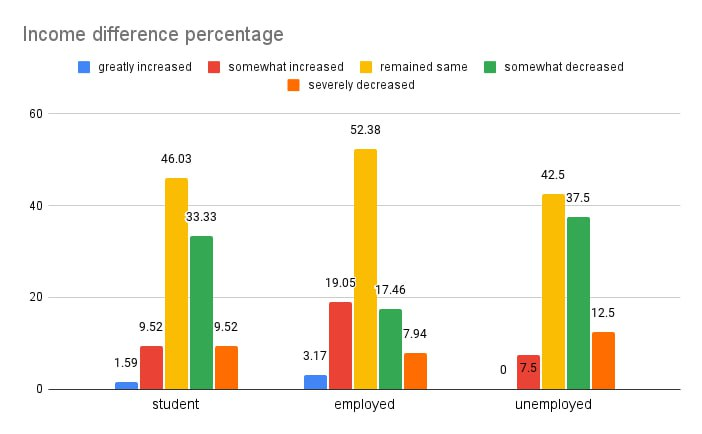
\includegraphics[width=0.9\linewidth]{IMAGES/Image 34.jpeg}
	\caption{Percentage of Differences in Incomes}
	\label{G34}
\end{figure}
$$\textit{Student($126$) | Employed($63$) | Unemployed($40$)}$$

\ 

The bar chart provides an overview of income change percentages across three distinct categories of individuals: \textit{students, employed individuals, and the unemployed}. The income change percentages are divided into five groups: "\textbf{Greatly Increased}", "\textbf{Somewhat Increased}", "\textbf{Remained Same}", "\textbf{Somewhat Decreased}", and "\textbf{Severely Decreased}".

\ 

In the case of students, $1.59\%$ experienced a significant increase in income, while $9.52\%$ observed a moderate rise. A substantial majority of students $(46.03\%)$ maintained a consistent income level, with approximately $33.33\%$ facing a moderate decrease and $9.52\%$ encountering a substantial reduction.

\ 

Among employed individuals, $3.17\%$ saw a notable increase in income, and $19.05\%$ experienced a moderate rise. The largest portion of employed individuals $(52.38\%)$ sustained a steady income level, while around $17.46\%$ observed a moderate decline, and $7.94\%$ faced a substantial reduction.

\

For unemployed individuals, none experienced a significant increase, and $7.5\%$ observed a moderate rise. A significant majority $(42.5\%)$ maintained a consistent income level, while around $37.5\%$ experienced a moderate decrease, and $12.5\%$ encountered a substantial reduction.

\ 

Analyzing these figures reveals that the largest percentage of employed individuals $(52.38\%)$ maintained a steady income level, surpassing both students $(46.03\%)$ and unemployed individuals $(42.5\%)$. Moreover, a notable portion of students $(33.33\%)$ faced a moderate decrease in income, exceeding the corresponding percentages for employed and unemployed individuals.

\ 

It is noteworthy that the percentage of unemployed individuals experiencing any level of increased income $(7.5\%)$ is notably lower compared to students $(11.11\%)$ and employed individuals $(22.22\%)$. This breakdown of income change percentages across employment categories provides insights into the varying income dynamics experienced by different groups based on their employment status.

\newpage

\subsection{Income Difference between Pre-Pandemic\\ and Post-Pandemic Situation}

\begin{figure}[h!]
	\centering
	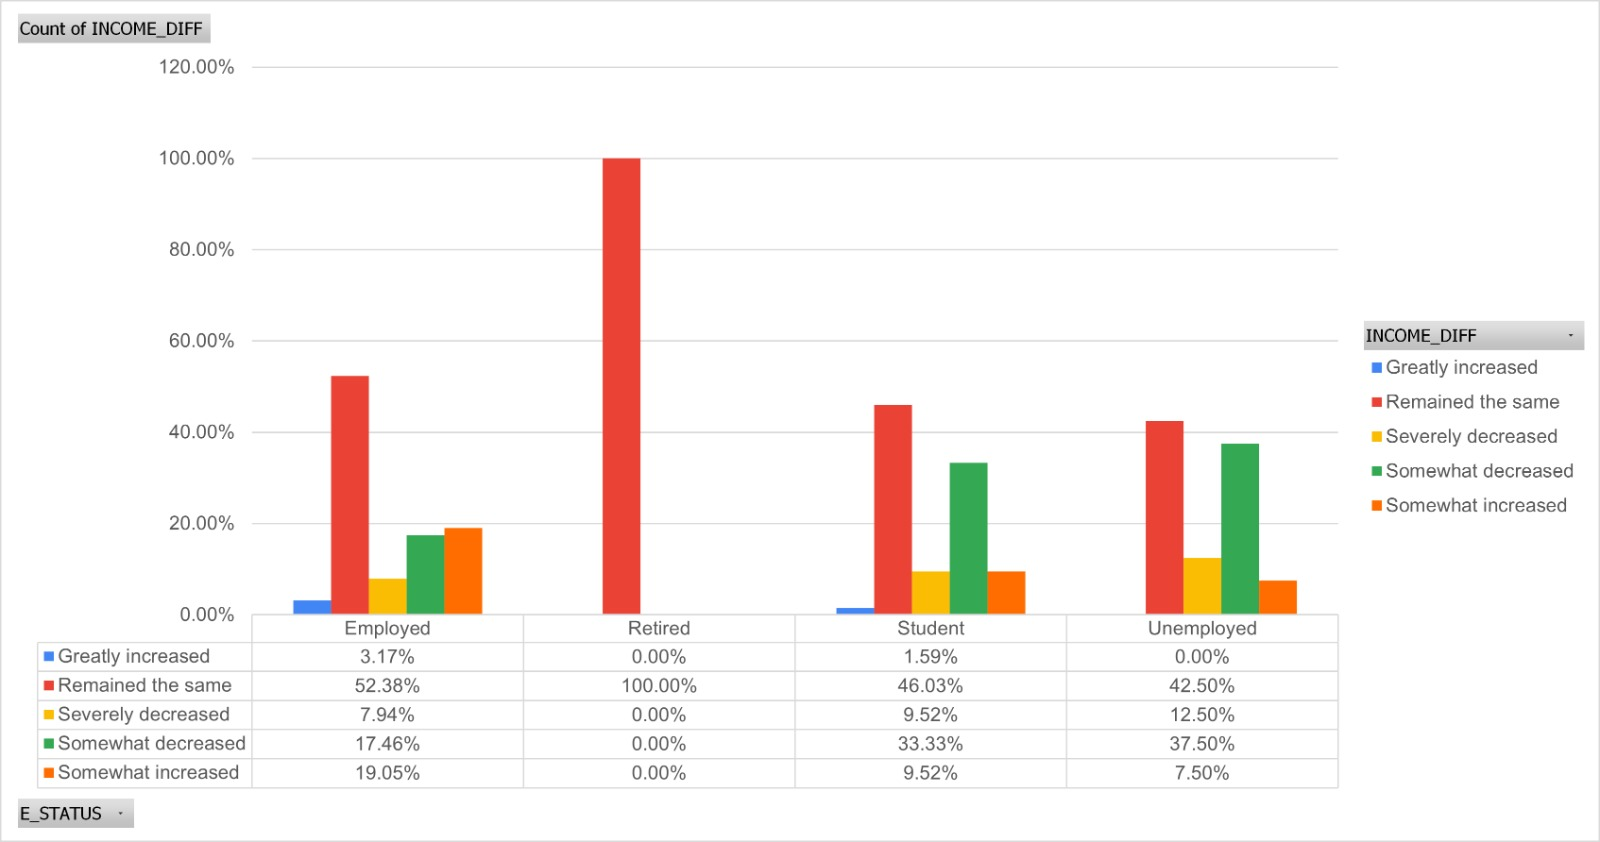
\includegraphics[width=0.8\linewidth]{IMAGES/Image 5.jpg}
	\caption{Difference in Incomes}
	\label{G5}
\end{figure}
$$\textit{Employed($63$) | Retired($1$) | Student($126$) | Unemployed($40$)}$$

\ 

The bar graph in Figure \ref{G5} illustrates the difference in incomes between the pre-pandemic and post-pandemic period for participants with different employment status. It is measured in percentage. Overall it can be observed that the income remained almost same or somewhat decreased in each employment category.

\ 

Almost half of the participants with the employed, student and unemployed status had their salary unaffected and also the retired one. In the group of student and unemployed ones, $1/3^{rd}$  portion and among employed ones $17.46\%$  had slight decrement in their income. Only a very small part in employed and student category claimed great increase in their income. About $10\%$ participant's salary got critically decreased. 

\newpage

\section{Dependence on Cooked Food Delivery System}

\begin{figure}[h!]
	\centering
	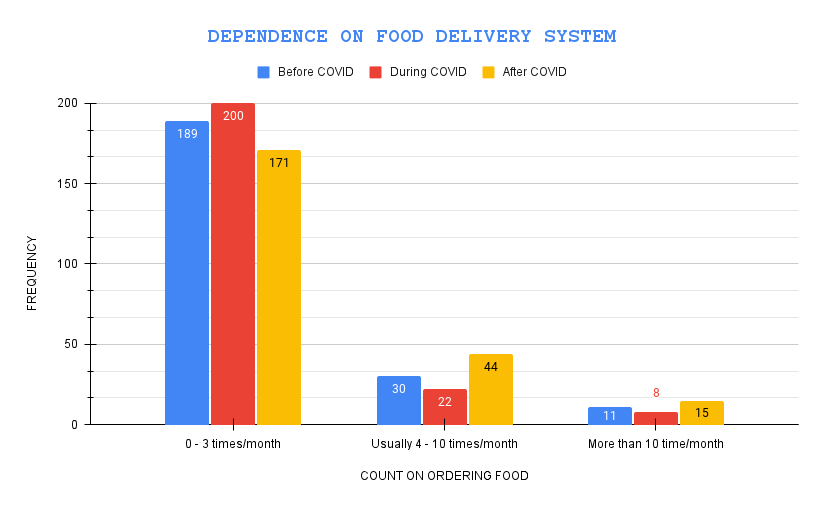
\includegraphics[width=0.8\linewidth]{IMAGES/Image 13.png}
	\caption{Dependence on Cooked Food Delivery System}
	\label{G13}
\end{figure}

\ 

\begin{figure}[h!]
	\centering
	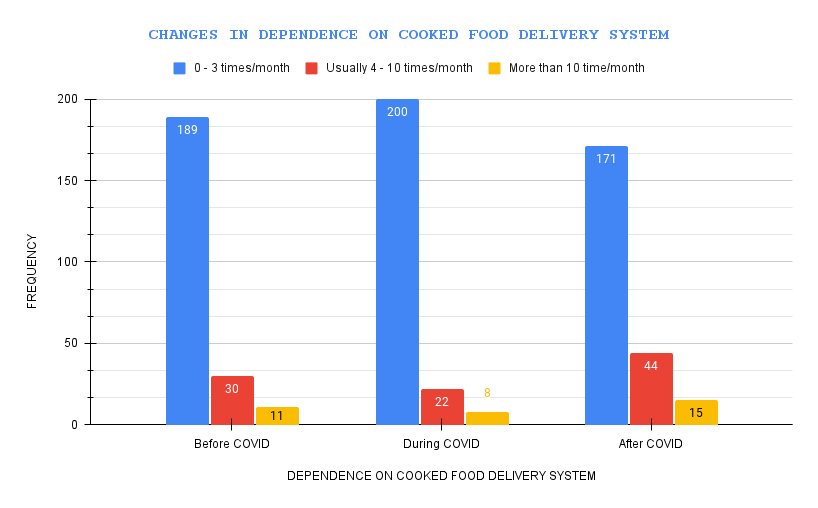
\includegraphics[width=0.8\linewidth]{IMAGES/Image 14.png}
	\caption{Dependence on Cooked Food Delivery System}
	\label{G14}
\end{figure}

Figure \ref{G13} and Figure \ref{G14} illustrate a comparison between the number of times the participants ordered food online in a month before, during and after COVID-19. The majority of participants, regardless of the pandemic, exhibit a trend of ordering food online 0-3 times per month.

\newpage

\subsection{Changes in Online Food ordering frequency}

\begin{figure}[h!]
	\centering
	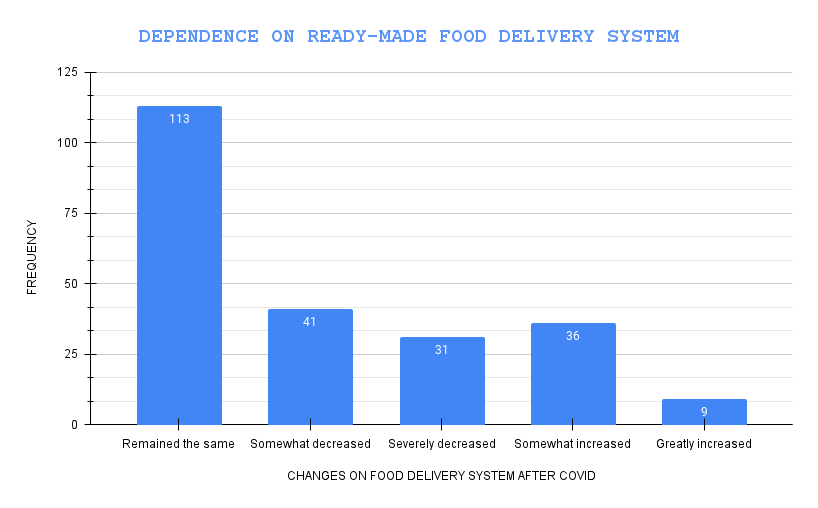
\includegraphics[width=0.9\linewidth]{IMAGES/Image 15.png}
	\caption{Dependence on Cooked Food Delivery System}
	\label{G15}
\end{figure}

\

The data provided in Figure 4.3 illustrates the frequency dependence on ready-made food delivery systems. The majority of the respondents reported that their dependence on ready-made food delivery remained the same, while a smaller percentage indicated a somewhat decreased dependence and an even smaller percentage reported a severe decrease in dependence. Conversely, some respondents mentioned a somewhat increased dependence on ready-made food delivery, but the number of responses with greatly increased dependence has been very low.

\ 

This data mostly indicates two aspects of thought processes adapted by people during the COVID-19 Lockdown period. A significant number of families believed that the Virus could be carried through right into the house with the ready-made food despite all the precaution and contactless delivery etc. Hence, the chances of contamination may increase. Therefore, they somewhat decreased ordering ready-made food. On the other hand, a significant amount of people felt the need of ordering ready-made food more often than before. This may be due to lack of availability of raw cooking materials during the Lockdown period, or it might be safe to say that a few got addicted to an easier lifestyle that the pandemic offered.

\newpage

\subsection{Changes in Online Food ordering frequency \\ across different employment Categories}
\begin{figure}[h!]
	\centering
	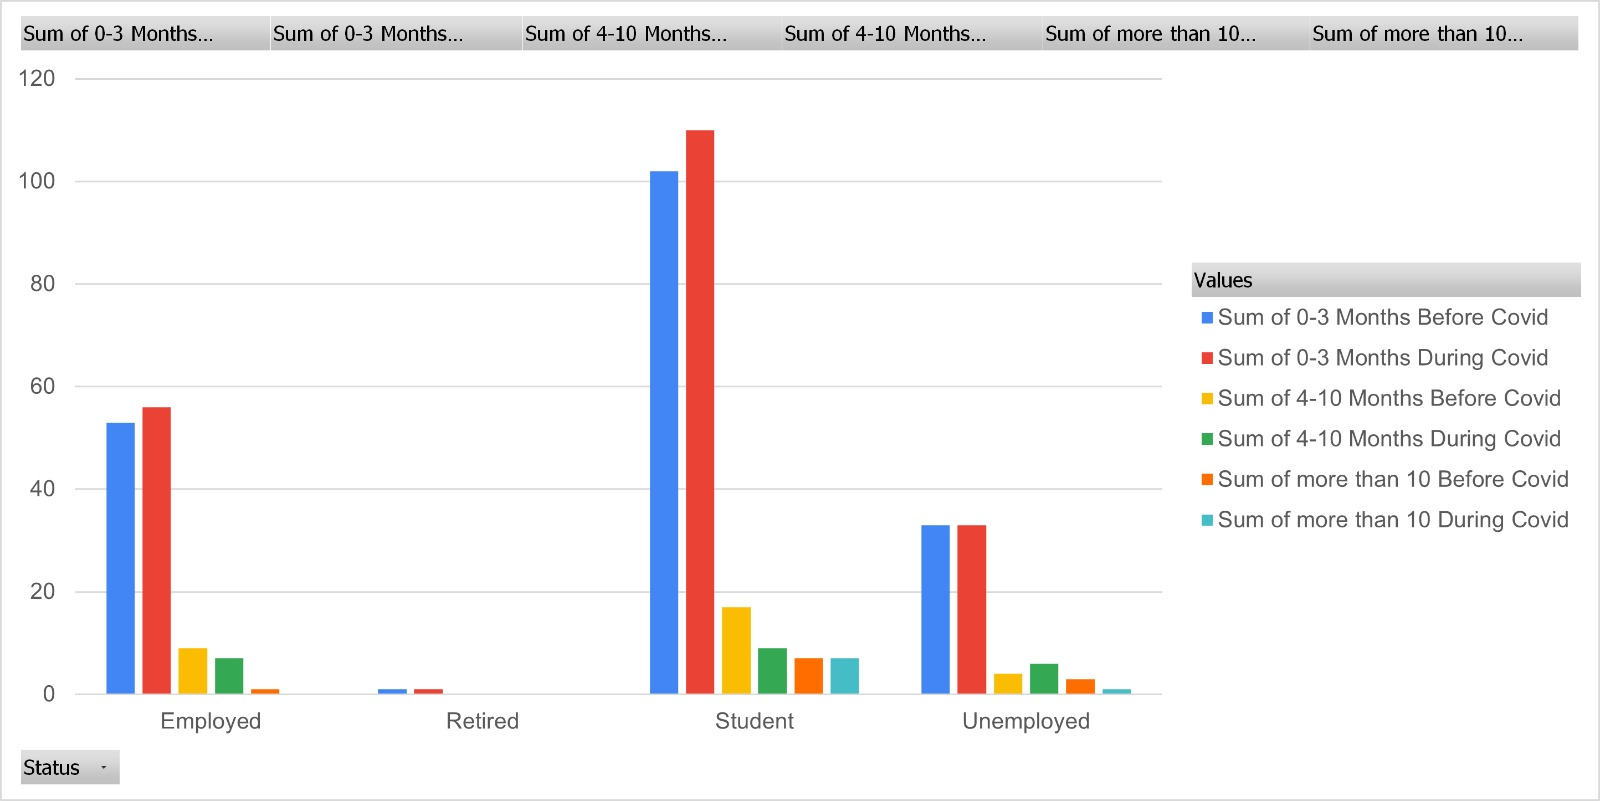
\includegraphics[width=0.9\linewidth]{IMAGES/Image 6.jpg}
	\caption{Dependence on Cooked Food Delivery System}
	\label{G6}
\end{figure}
$$\textit{Employed($63$) | Retired($1$) | Student($126$) | Unemployed($40$)}$$

\ 

Figure \ref{G6} represents the change in ‘Dependence on cooked-food delivery system’ due to pandemic for participants corresponding to several employment status. It is measured in corresponding frequency. 

\ 

From the mere observation, it can be seen that there has been some upward trend in the \textbf{“0-3 times per month}” segment among the student and employed participants. Whereas the no. of unemployed and retired ones in this segment remained same as before COVID.\\ \\
The no. of students and employed persons in the “\textbf{4-10 times per month}” segment gets slightly decreased while the no. Of unemployed ones in this segment got slightly increased.

\

In the “\textbf{More than 10 times per month}” the students did not show any change of habit, while employed and unemployed ones reduced their order frequency. It should also be noted that there has been lest no. Of participants in this segment during COVID as well as before COVID. 

\newpage

\section{Vaccination Status}

\begin{figure}[h!]
	\centering
	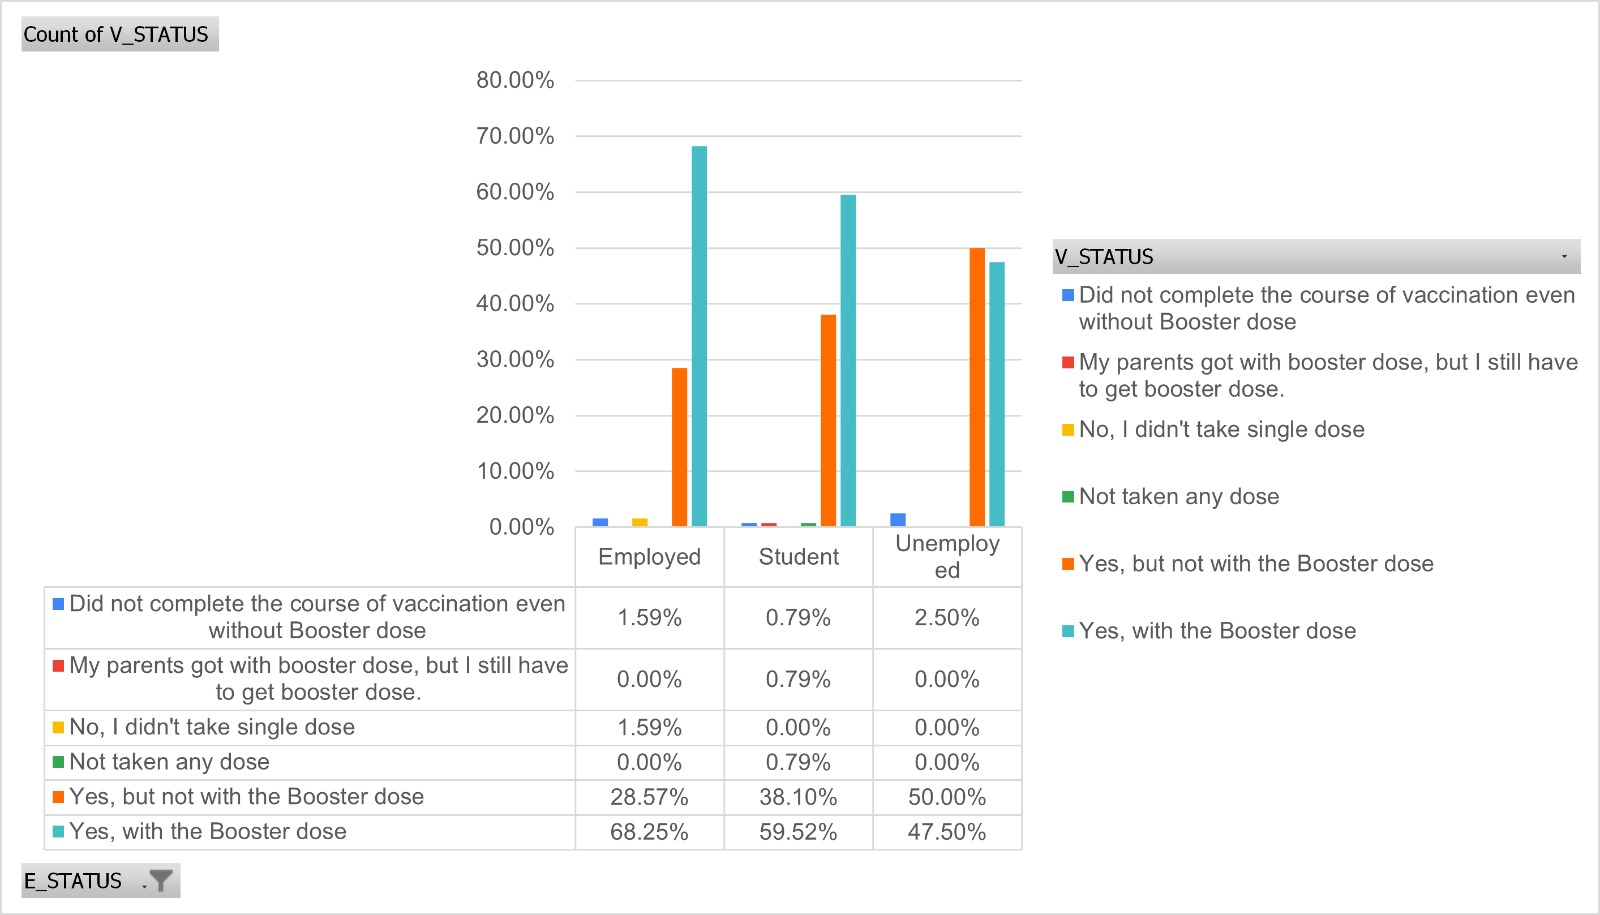
\includegraphics[width=0.9\linewidth]{IMAGES/Image 7.jpg}
	\caption{Vaccination Status}
	\label{G7}
\end{figure}
$$\textit{Employed($63$) | Retired($1$) | Student($126$) | Unemployed($40$)}$$

\ 

The bar graph in Figure \ref{G7} illustrates the vaccination status for participants with different employment condition. It has been measured in percentage.

\ 

There is $1.59\%$ employed participants who did not take any dose and a same portion with incomplete course of vaccination.  The majority of employed participants $(68.25\%)$ finished the vaccination with booster dose and $28.57\%$ without booster dose.

\

It can be observed that a very small portion of students either did not take the booster dose or  any dose. About $59.52\%$ of students got properly vaccinated and the remaining $38.10\%$ are to be vaccinated with the booster dose.

\

Among the unemployed participants only $2.50\%$ did not complete the vaccination process. While half of them got vaccinated without booster dose, $47.5\%$ completed the vaccination with booster dose.

\

It can be seen that almost all the participants are either fully vaccinated with booster dose or without booster dose.

\

\newpage

\section{Medical Expenses}

\begin{figure}[h!]
	\centering
	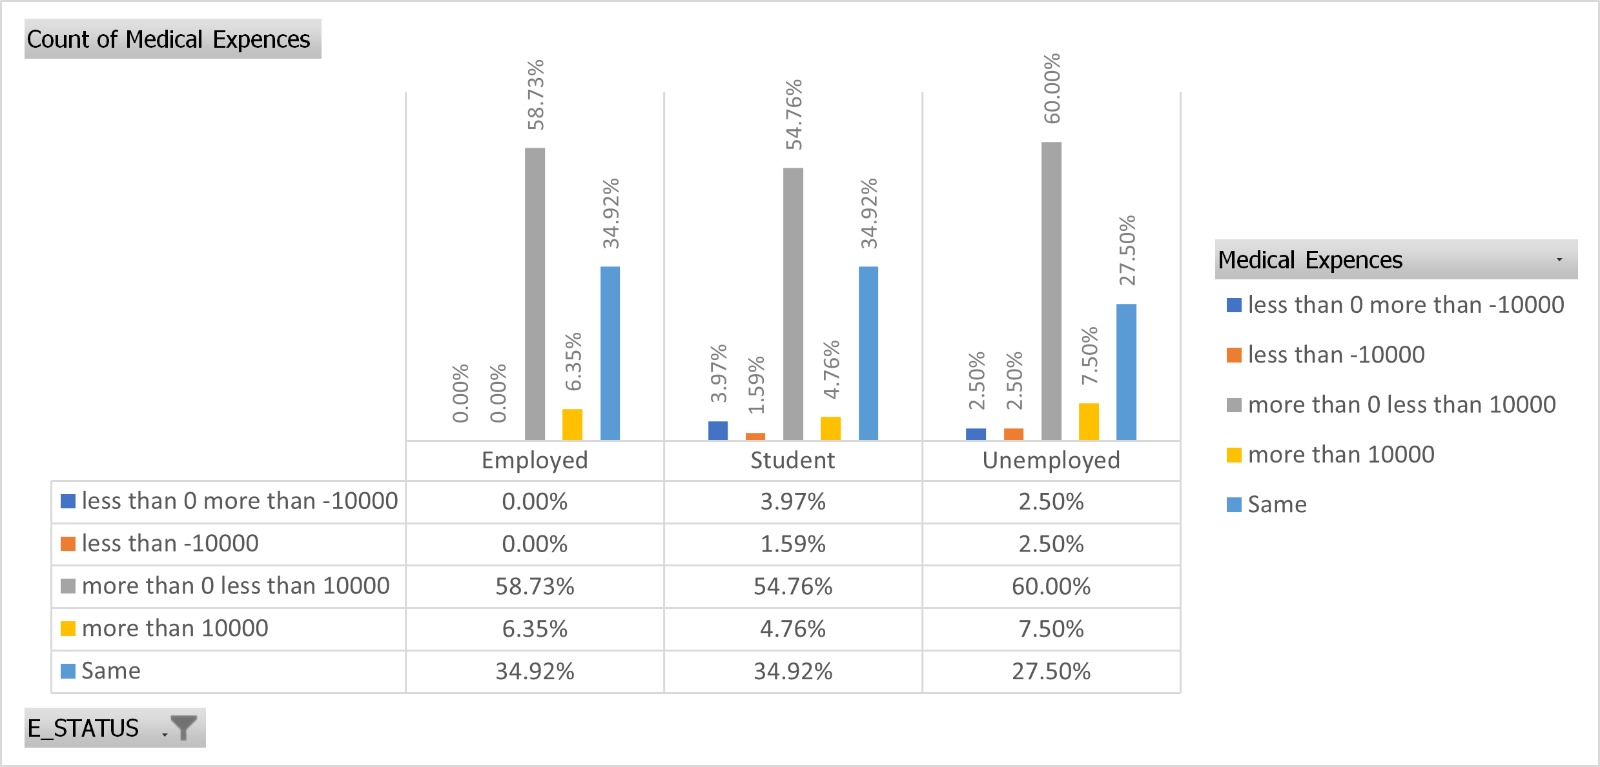
\includegraphics[width=0.85\linewidth]{IMAGES/Image 8.jpg}
	\caption{Count of Medical Expenses}
	\label{G8}
\end{figure}
$$\textit{Employed($63$) | Retired($1$) | Student($126$) | Unemployed($40$)}$$

\ 

Figure \ref{G8} shows that none of the employed candidates' medical expenses for their family members decreased by more than $10,000$ after the pandemic. Meanwhile, $0\%$ of employed candidates experienced a decrease between zero and $10,000$. About $6.35\%$ of employed candidates reported an increase of more than $10,000$ in medical expenses for their family, while $58.73\%$ reported an increase between zero and $10,000$. Additionally, $34.92\%$ of employed candidates stated that medical expenses for their family remained unchanged after the pandemic.

\

Among students, $1.59\%$ reported a decrease of more than $10,000$ in medical expenses for their family after the pandemic, while $3.97\%$ reported a decrease between zero and $10,000$. About $4.76\%$ of students experienced an increase of more than $10,000$, and $54.76\%$ reported an increase between zero and $10,000$. Furthermore, $34.92\%$ of students mentioned that medical expenses for their family remained unchanged after the pandemic.

\

For unemployed candidates, $2.50\%$ reported a decrease of more than $10,000$ in medical expenses for their family, and $2.50\%$ reported a decrease between zero and $10,000$. About $7.50\%$ of unemployed candidates experienced an increase of more than $10,000$, while $60\%$ reported an increase between zero and $10,000$. Additionally, $27.50\%$ of unemployed candidates stated that medical expenses for their family remained unchanged after the pandemic.
\newpage 

\section{Weight Difference}

\begin{figure}[h!]
	\centering
	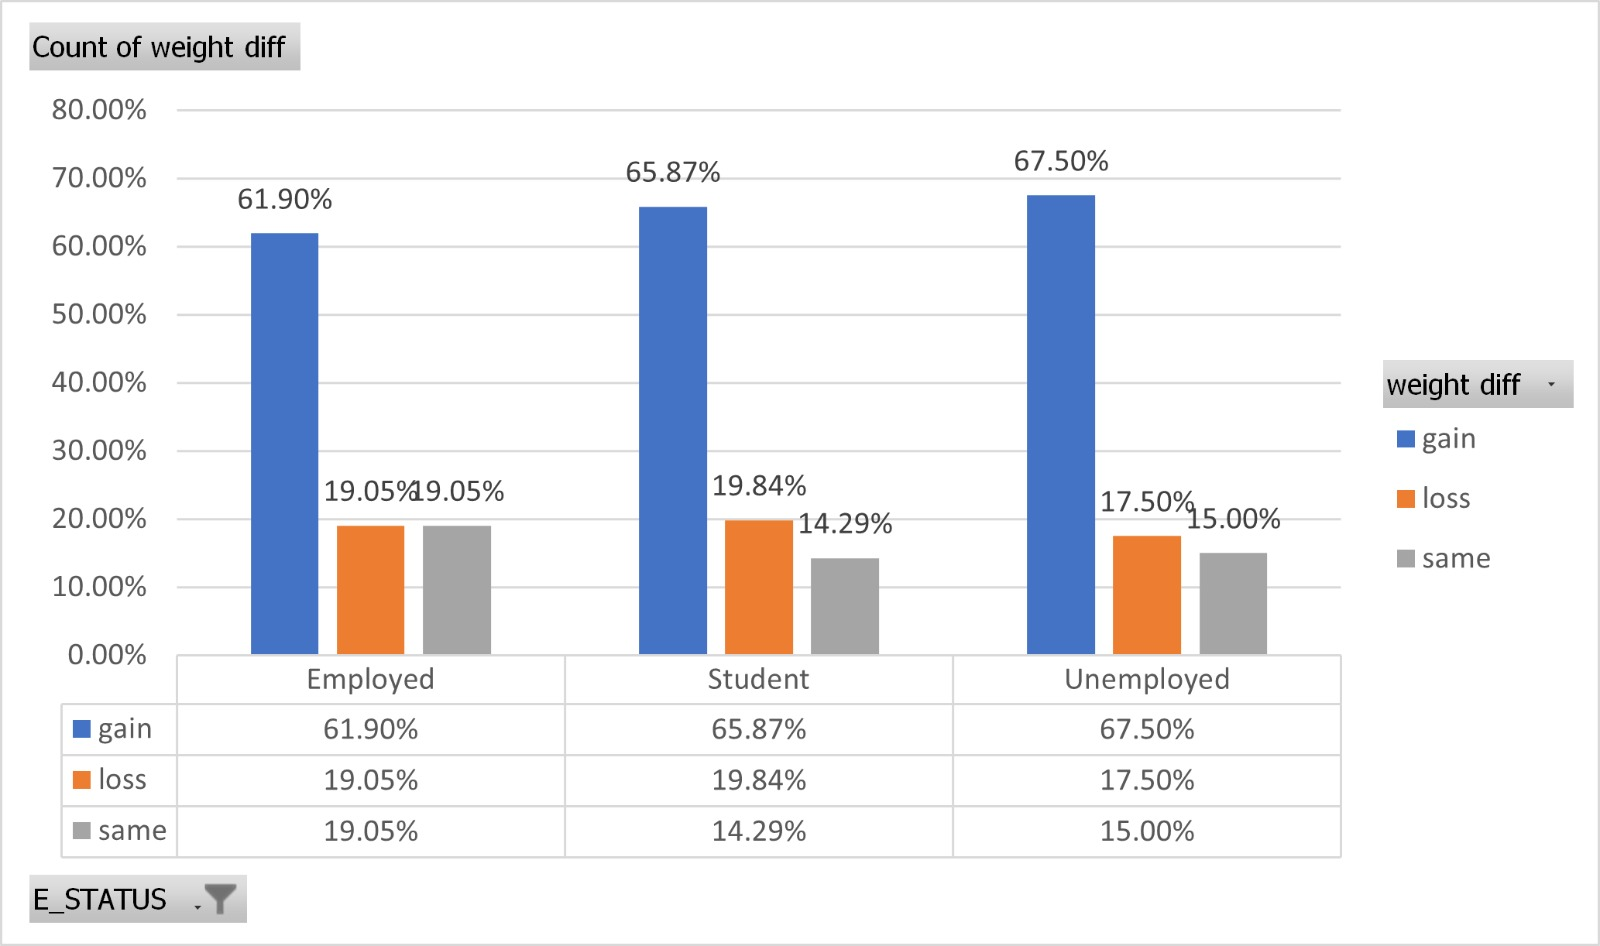
\includegraphics[width=0.9\linewidth]{IMAGES/Image 9.jpg}
	\caption{Weight Difference between Pre and Post-Pandemic Situations}
	\label{G9}
\end{figure}
$$\textit{Employed($63$) | Retired($1$) | Student($126$) | Unemployed($40$)}$$

\ 

Figure \ref{G9} shows that among employed candidates $61.90\%$ gained weight during the pandemic (COVID-19), $19.05\%$ lost weight, and the weight remained the same for $19.05\%$.

\ 

Among students, $65.87\%$ gained weight during the pandemic (COVID-19), $19.84\%$ lost weight, and the weight remained the same for $14.29\%$.

\ 

Among unemployed candidates, $67.50\%$ gained weight during the pandemic (COVID-19), $17.50\%$ lost weight, and the weight remained the same for $15.00\%$.


\newpage

\section{Outdoor Socialization}

\subsection{Going Outside}

\begin{figure}[h!]
	\centering
	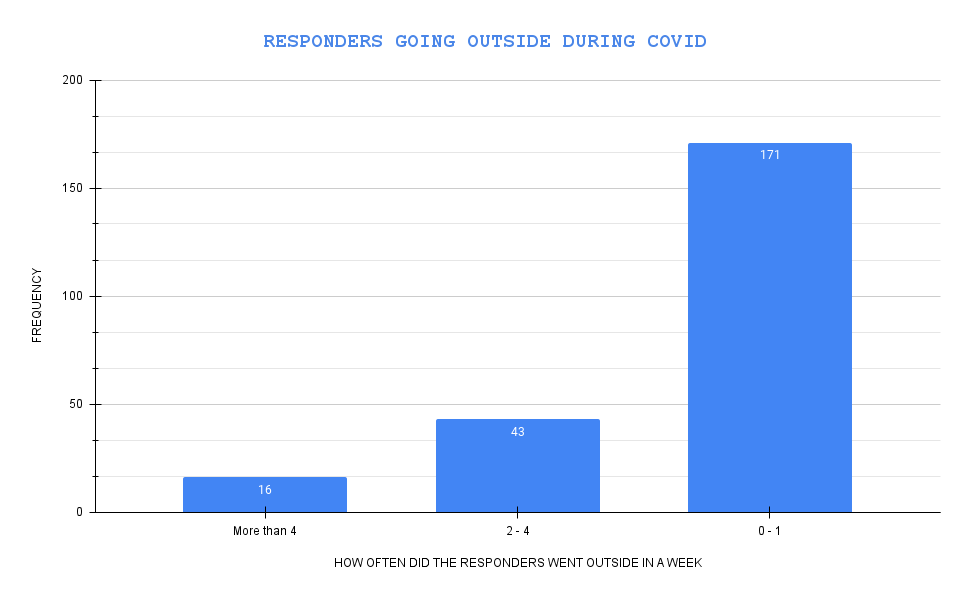
\includegraphics[width=0.6\linewidth]{IMAGES/Image 22.png}
	\caption{Going Outside}
	\label{G22}
\end{figure}

Due to the impact of COVID-19, the frequency of going out has undergone a substantial change. From figure \ref{G22} we see that among the $230$ participants surveyed, $171$ individuals reported going out at most once a week during the pandemic.

\subsection{Social Interaction}

\begin{figure}[h!]
	\centering
	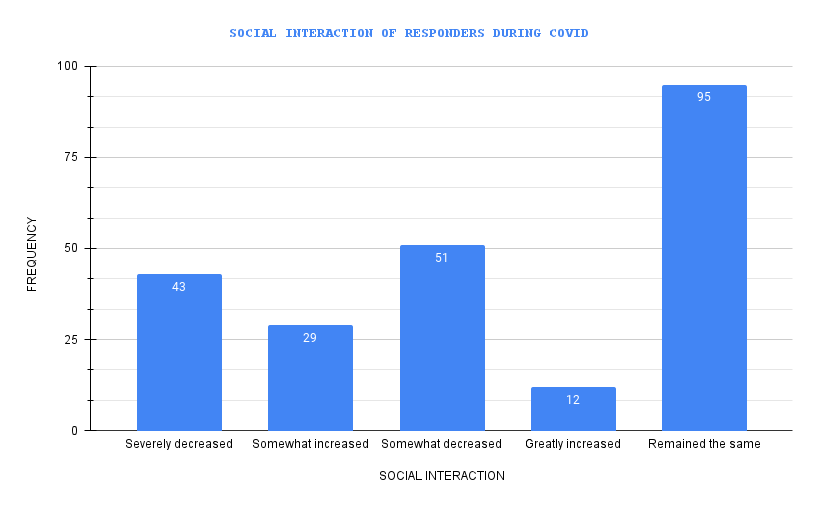
\includegraphics[width=0.6\linewidth]{IMAGES/Image 23.png}
	\caption{Social Interaction}
	\label{G23}
\end{figure}

Clearly it has also affected social interaction. Figure \ref{G23} illustrates that the social interaction of $43$ people has markedly diminished, while $29$ people have experienced a modest increase. For $51$ individuals, social engagement has somewhat decreased, whereas $12$ people have seen a notable rise in their social interactions. Remarkably, the social interactions of $95$ people have remained unchanged.


\newpage


\subsection{Precautionary Measures taken up by Individuals}

\begin{figure}[h!]
    \centering
    \begin{subfigure}{0.45\linewidth}
        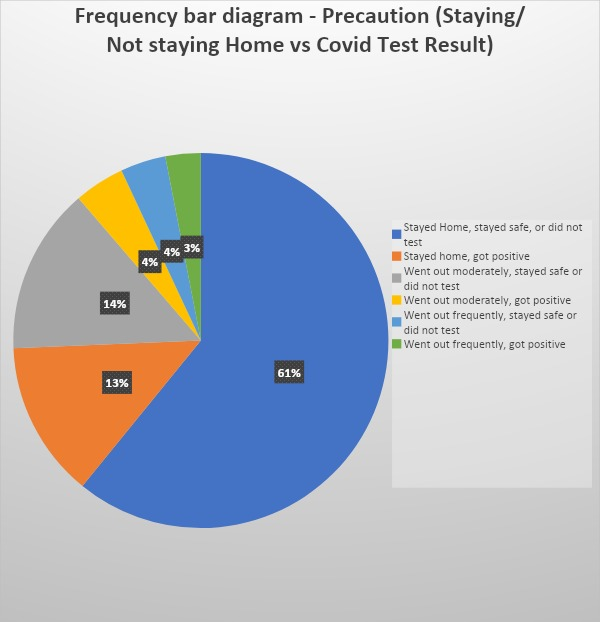
\includegraphics[width=\linewidth]{IMAGES/Image 29.jpeg}
        \caption{Precautions taken}
        \label{G29}
    \end{subfigure}
    \hfill
    \begin{subfigure}{0.45\linewidth}
        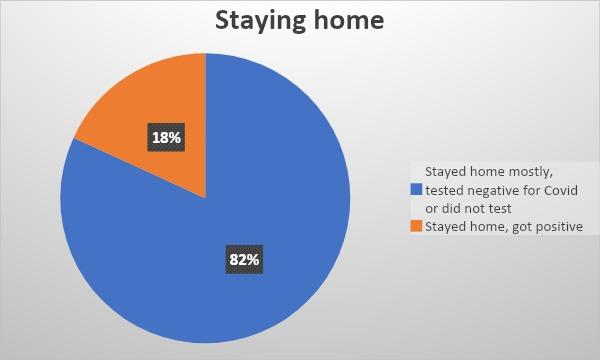
\includegraphics[width=\linewidth]{IMAGES/Image 30.jpeg}
        \caption{Staying at home}
        \label{G30}
    \end{subfigure}
    
    \begin{subfigure}{0.45\linewidth}
        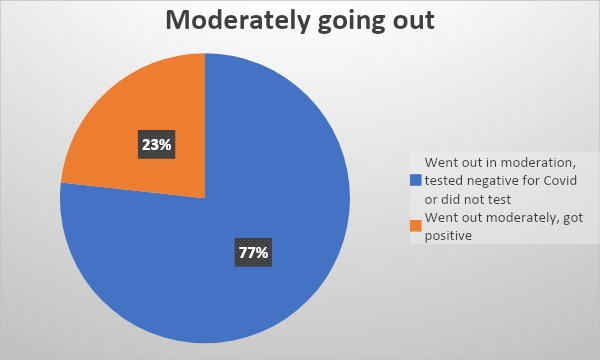
\includegraphics[width=\linewidth]{IMAGES/Image 31.jpeg}
        \caption{Moderately going out}
        \label{G31}
    \end{subfigure}
    \hfill
    \begin{subfigure}{0.45\linewidth}
        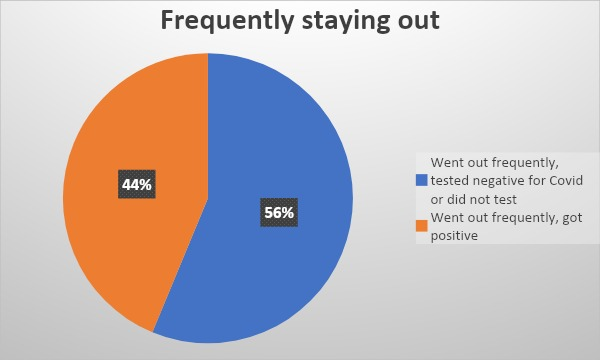
\includegraphics[width=\linewidth]{IMAGES/Image 32.jpeg}
        \caption{Frequently going out}
        \label{G32}
    \end{subfigure}

    \caption{Precautions taken in four images}
    \label{all_images}
\end{figure}


\ 

The pie charts \ref{all_images} above provides an overview of the percentage distribution of the sample population across different categories related to staying at home during the COVID-19 pandemic. Approximately $61\%$ of individuals mostly stayed at home and remained untouched by COVID infection. Another $14\%$ of individuals contracted COVID while staying at home for unknown reason. Additionally, about $14\%$ of the population ventured out moderately during the COVID pandemic and either stayed negative or did not get tested. A small percentage $4\%$ of individuals who went out moderately got infected by the COVID virus. The percentage of people who frequently went out was small, and $4\%$ of them either stayed safe or did not get tested. Only $3\%$ of the population that went out frequently got infected with COVID.

\newpage 

Analyzing the pie chart, it becomes evident that staying at home played a crucial role in preventing the spread of COVID-19. Only $18\%$ of the sample population staying at home were infected, while $82\%$ remained mostly safe. The next pie chart illustrates the infection spread due to moderate outings, showing that $23\%$ of the sample population got infected due to moderate outings during the COVID pandemic. In the last pie chart, the results of frequently staying out are shown to contribute significantly to the increase in the spread of COVID infection, rising to $44\%$. This suggests that going out frequently led to a higher risk of contamination.

\ 

The insights derived from the data are noteworthy. Staying at home emerged as a significant factor in preventing the spread of COVID and getting infected, as evidenced by the relatively low infection rate of $18\%$. However, as people went out moderately from home, the rate of infection and positive cases increased by $5\%$, indicating a relatively lower impact of moderate outings. Overall, the survey depicts that frequently staying out is a major factor contributing to the spread of COVID. Due to this factor, the infection rate rose by $26\%$ compared to staying at home.

\newpage 

\section{Screen-time}

\subsection{Changes in Screen time}

\begin{figure}[h!]
	\centering

 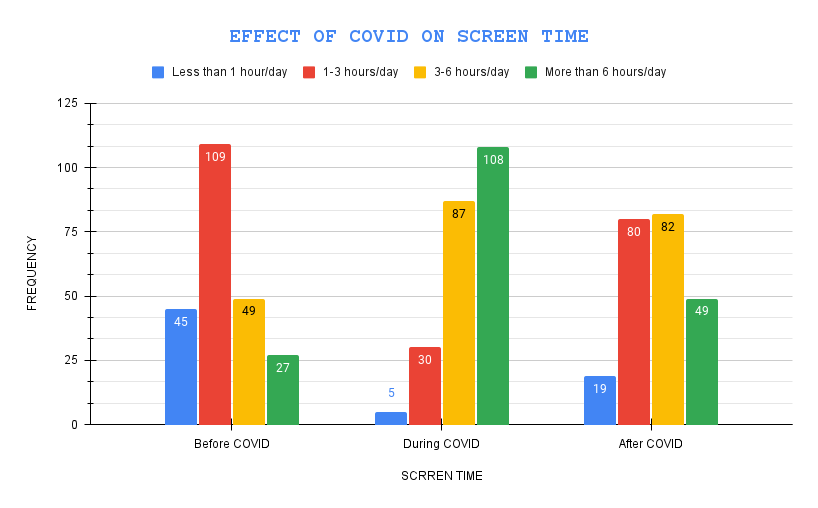
\includegraphics[width=0.75\linewidth]{IMAGES/Image 16.png}
	\caption{Changes in Screen-time}
	\label{G16}
\end{figure}

The information presented in Figure \ref{G16} illustrates a comparison of daily screen time during distinct time periods—before, during and after the COVID-19 pandemic.

\subsection{Screen time Frequency}

\begin{figure}[h!]
	\centering
	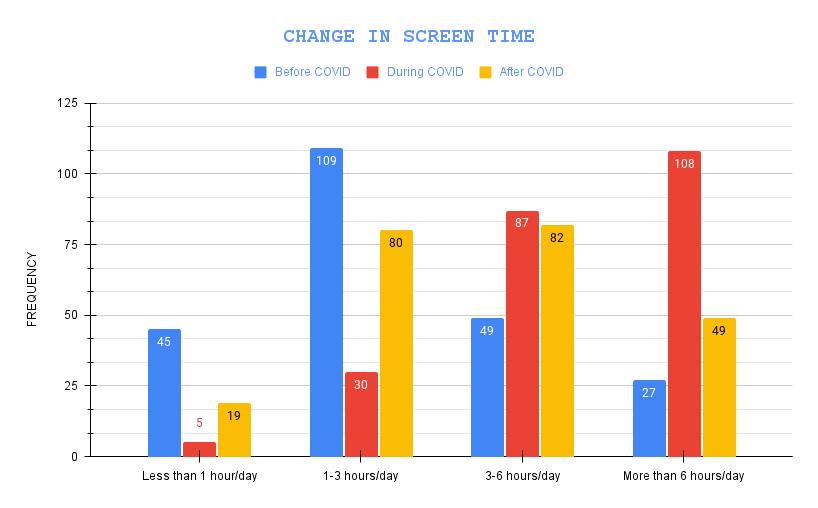
\includegraphics[width=0.75\linewidth]{IMAGES/Image 17.png}
	\caption{Screen-time Frequency}
	\label{G17}
\end{figure}


Figure \ref{G17} presents a visual representation comparing the number of people having a particular limit of screen time before, during and after the COVID-19.

\newpage 

\subsection{Screen time Percentage}

\begin{figure}[h!]
	\centering
	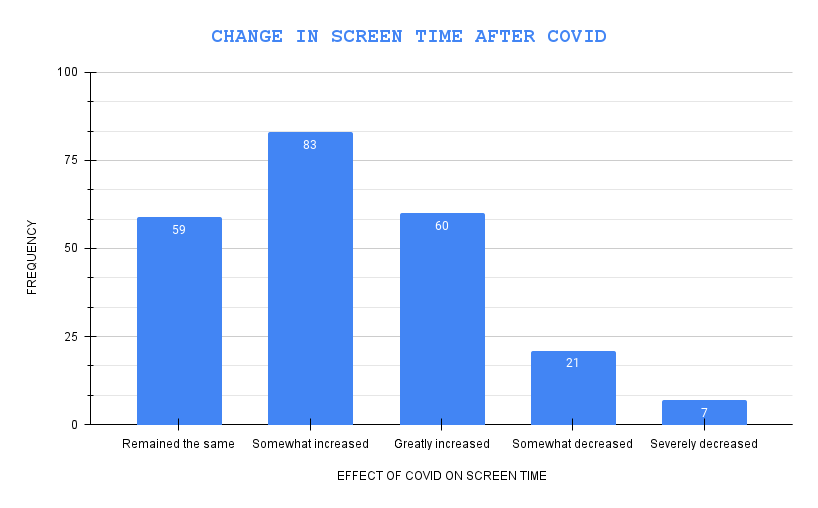
\includegraphics[width=0.79\linewidth]{IMAGES/Image 18.png}
	\caption{Screen-time Percentage}
	\label{G18}
\end{figure}
Figure \ref{G18} shows that for majority of the participants the screen time has somewhat increased during COVID 19. Before COVID-19, the majority of participants reported engaging in screen time for \textbf{1-3 hours} per day. However, with the advent of the pandemic, there has been a notable and significant increase in the number of individuals spending more than \textbf{6 hours per day} on screens. Also, the proportion of people with \textbf{less than 1 hour} of screen time per day during this period has diminished considerably. Post-COVID-19, a substantial portion of participants now falls within the range of \textbf{1-6 hours} of daily screen time.

\begin{figure}[h!]
	\centering
	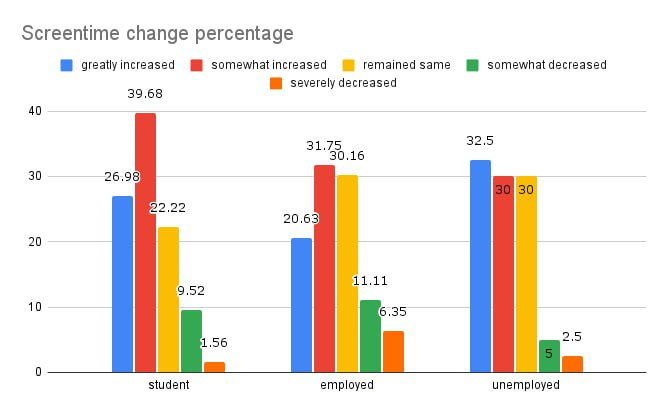
\includegraphics[width=0.79\linewidth]{IMAGES/Image 10.jpeg}
	\caption{Screen-time Percentage of different Employment Categories}
	\label{G10}
\end{figure}

\newpage

Figure \ref{G10} represents the screen time changes for different categories of people during COVID-19. It indicates that across all categories, screen time has somewhat increased to a large extent.

\ 

For students, employees and unemployed, the percentages are $39.68\%$, $31.75\%$ and $30\%$, respectively. Additionally, a significant percentage increase is observed for people from different categories, with percentages of $26.98\%$, $20.63\%$ and $32.5\%$ for \textit{students, employees and unemployed} respectively.

\

The data also reveals that screen time has remained the same for a substantial number of people. An interesting observation is that among those experiencing a significant increase in screen time, the proportion is highest for unemployed individuals, followed by students and employed individuals in decreasing order.

\section{Mental Health}

\subsection{Mental Health conditions}

\begin{figure}[h!]
	\centering
	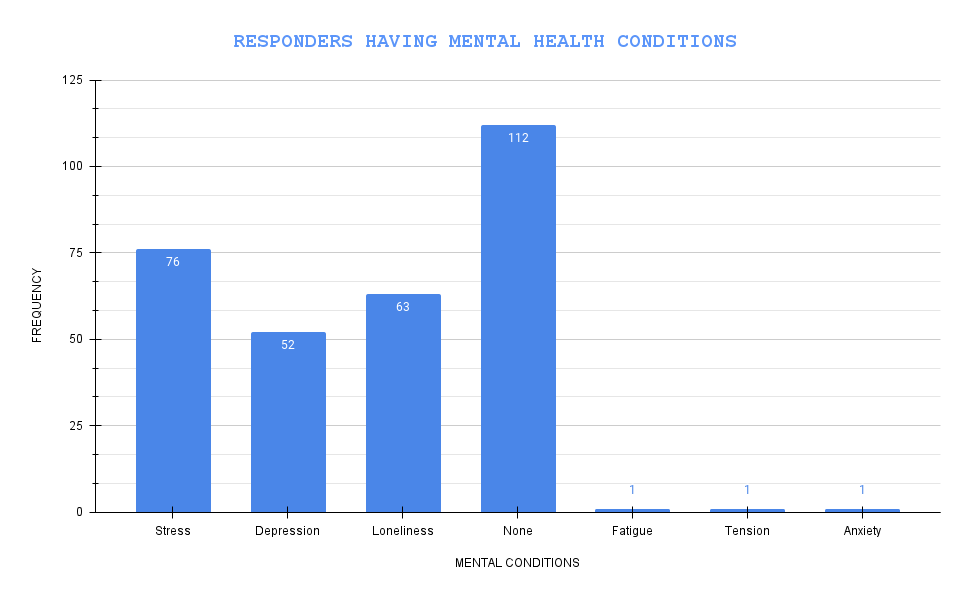
\includegraphics[width=0.9\linewidth]{IMAGES/Image 12.png}
	\caption{Mental Health Conditions}
	\label{G12}
\end{figure}

\

Figure \ref{G12} shows the number of responders having mental health conditions during COVID-19 pandemic. The predominant conditions reported were stress, loneliness and depression, affecting $76$, $63$ and $52$ individuals, respectively. Noteworthy outliers included cases of fatigue, tension and anxiety. It is important to highlight that a substantial proportion of participants did not experience any mental health issues during this challenging time.

\newpage

\subsection{Mental Health across different Employment categories}

\begin{figure}[h!]
	\centering
	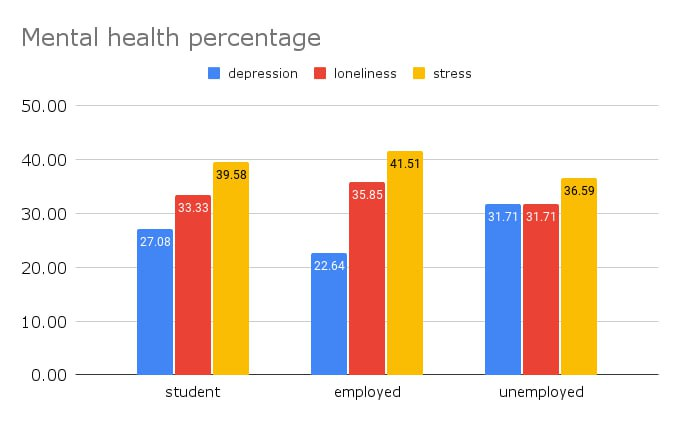
\includegraphics[width=0.9\linewidth]{IMAGES/Image 11.jpeg}
	\caption{Mental conditions across different Employment Categories}
	\label{G11}
\end{figure}
$$\textit{Employed($63$) | Retired($1$) | Student($126$) | Unemployed($40$)}$$

\ 

Figure \ref{G11} represents the mental health status of different categories during COVID-19.

\ 

It shows that 39.5\% of students, 41.51\% of employed individuals, and 36.59\% of unemployed persons were experiencing stress. A significant number of people were also dealing with loneliness, with rates of 33.33\% for students, 35.85\% for employed individuals, and 31.71\% for the unemployed. Additionally, 27.08\% of students, 22.64\% of employed individuals, and 31.71\% of unemployed persons have faced depression.

\

The above observations depict that almost everyone in all categories has gone through a mental health crisis. A sense of uncertainty and helplessness are the main reasons behind it. Loss of families, friends, jobs, and many more have pushed us towards another significant crisis—mental health.

\newpage

\section{Effects on Education System}

\begin{figure}[h!]
	\centering
	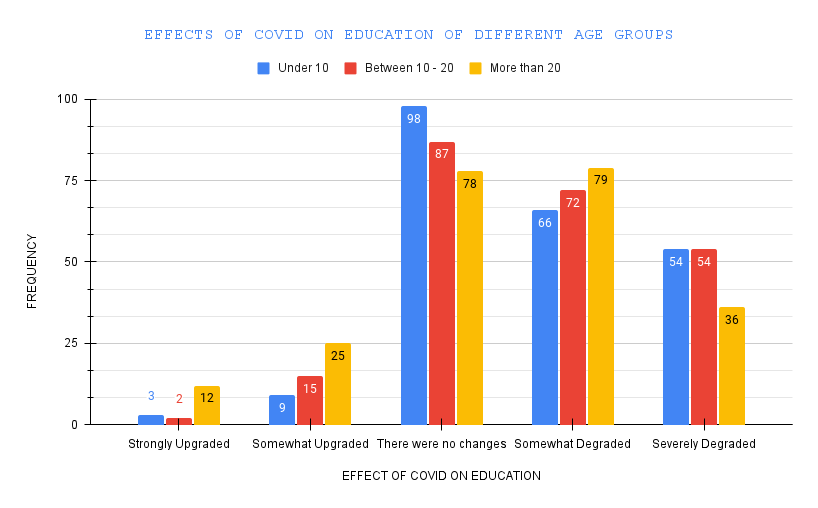
\includegraphics[width=1\linewidth]{IMAGES/Image 21.png}
	\caption{Effects on Education}
	\label{G21}
\end{figure}

\ 

Figure \ref{G21} provides insights into the impact of COVID-19 on the education of various age groups. 

\ 

In conclusion, the data indicate that education among children under the age of $10$ has either stayed consistent or has decreased in comparison to the pre-pandemic period. The quality of education has remained the same or has declined for children aged $10$ to $20$ and adult education has stayed stable or has deteriorated a bit.

\subsection{Association with any Institutional Activities}

Figure \ref{G24} displays the impact of the COVID-19 epidemic on responder's participation in institutional activities. Before the pandemic, the frequency of engagement stood at $84$, but during the pandemic, it soared to $146$. Subsequently, post-pandemic, the frequency dropped to $98$. This dynamic pattern demonstrates a significant increase in overall responders engagement during the pandemic. On the other hand, $54$ respondents, remained uninvolved in any institutional activity for the entire period.

\begin{figure}[h!]
	\centering
	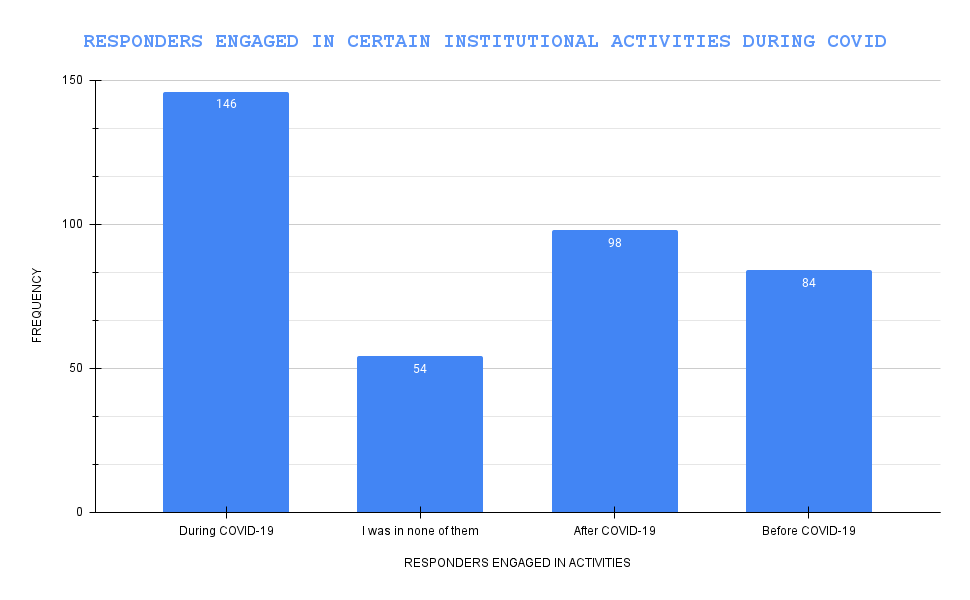
\includegraphics[width=0.9\linewidth]{IMAGES/Image 24.png}
	\caption{Institutional Activities}
	\label{G24}
\end{figure}

\section{Work from Home}

Figure \ref{G25} Among participant $73$ people used to work from home before the COVID-19 outbreak and after COVID-19 the number of people who worked from home has been increased to $87$.

\begin{figure}[h!]
	\centering
	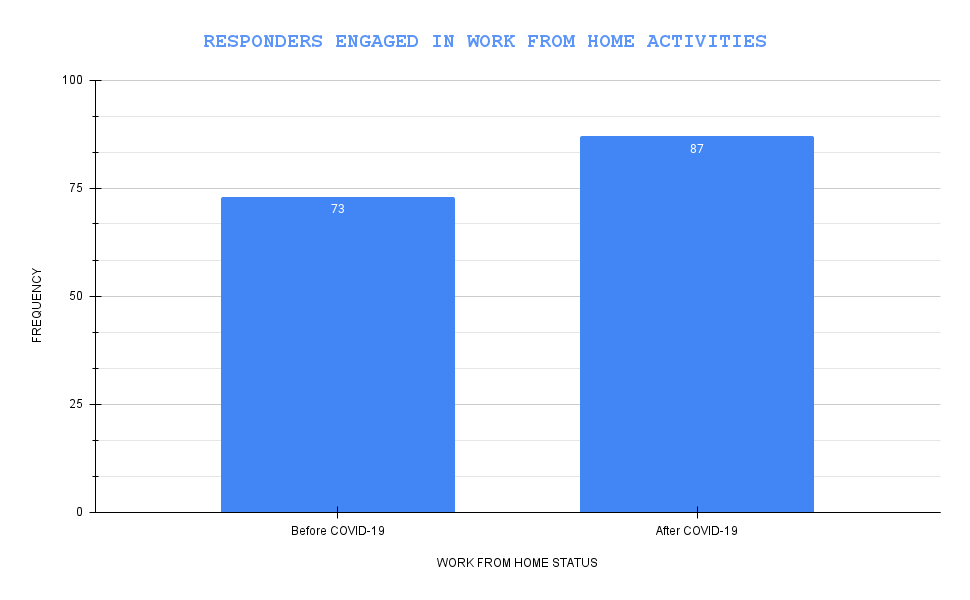
\includegraphics[width=0.9\linewidth]{IMAGES/Image 25.png}
	\caption{Work from Home}
	\label{G25}
\end{figure}

\newpage

\section{Healthy Habits taken up by Individuals}

\begin{figure}[h!]
	\centering
	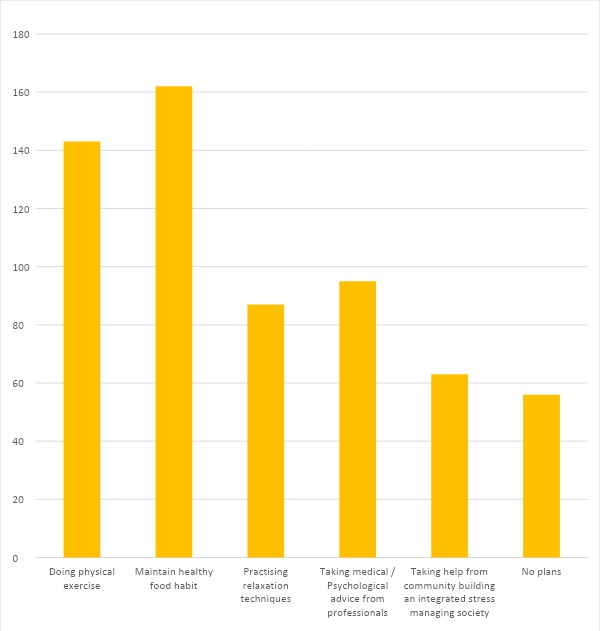
\includegraphics[width=0.9\linewidth]{IMAGES/Image 28.jpeg}
	\caption{Healthy Habits}
	\label{G28}
\end{figure}

Analyzing the healthy habits taken up by the individuals reveals some interesting trends among the $230$ participants. A significant $70.43\%$ express a desire to maintain a healthy food habit, emphasizing the importance placed on nutrition in their overall well-being. Additionally, $62.17\%$ are keen on incorporating regular physical exercises into their routines, highlighting a conscious effort to stay physically active for optimal health.

\

Furthermore, the data indicates that $37.82\%$ of participants are inclined towards practicing relaxation techniques, showcasing a recognition of the importance of mental well-being. Notably, $41.30\%$ express a preference for seeking medical or psychological advice from professionals, indicating a proactive approach to managing their health through expert guidance.

\

In an intriguing dimension, $27.39\%$ of individuals express a desire to seek support from their community in building an integrated stress management society to address the challenges posed by diseases. This reflects a community-oriented mindset in combating health issues collaboratively.

\

However, $24.34\%$ of the participants seem to lack pre-planning in adopting specific healthy habits. This highlights a potential area for intervention and education to raise awareness about the benefits of proactive health measures.

\

Insights drawn from the data underscore the prominence of individuals aiming to maintain both a healthy food habit and regular physical exercises, with percentages of $70.43\%$ and $62.17\%$, respectively. This dual focus on nutrition and physical activity suggests a holistic approach to health, particularly in the context of combating severe pandemics.

\

As we navigate the challenges of the current pandemic, it becomes evident that having hygiene plans in place is a proactive measure against potential future epidemics, such as the possibility of another COVID-19-like situation within the next 20 years. The importance of developing personal and community hygiene strategies cannot be overstated, as these measures play a crucial role in mitigating the spread of infectious diseases and fostering a healthier society overall.

\section{Proclivity for Physical Exercise - Before and After COVID-19}

\begin{figure}[h!]
	\centering
	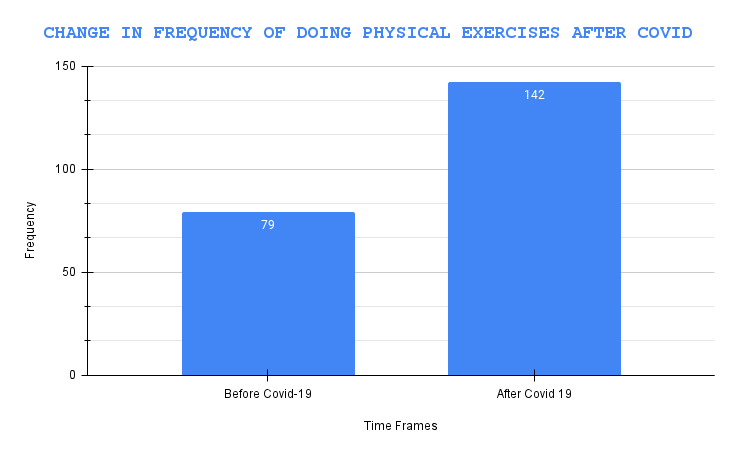
\includegraphics[width=0.9\linewidth]{IMAGES/Image 35.png}
	\caption{Physical Exercises after COVID-19}
	\label{G35}
\end{figure}

\ 

In the Bar diagram \ref{G35} illustrates findings from the aforementioned survey, showcasing the distinctions in physical exercise patterns before and after the onset of COVID-19. 

\

Based on the figure \ref{G35} depicting physical exercise frequency before and after COVID-19, it is evident that there was an increase in the frequency of physical exercise. Before COVID-19, the frequency was $79$, while after COVID-19, the frequency rose to $142$. This suggests a notable shift in exercise habits, with a higher number of individuals engaging in physical activities post-COVID-19 compared to the Pre-COVID-19 period. 

\

The increase in frequency may be attributed to various factors, such as heightened awareness of health, changes in daily routines, or a greater emphasis on physical well
being in response to the pandemic. 

\section{Evolving Impact of Widespread Sanitizer Use}

\begin{figure}[h!]
	\centering
	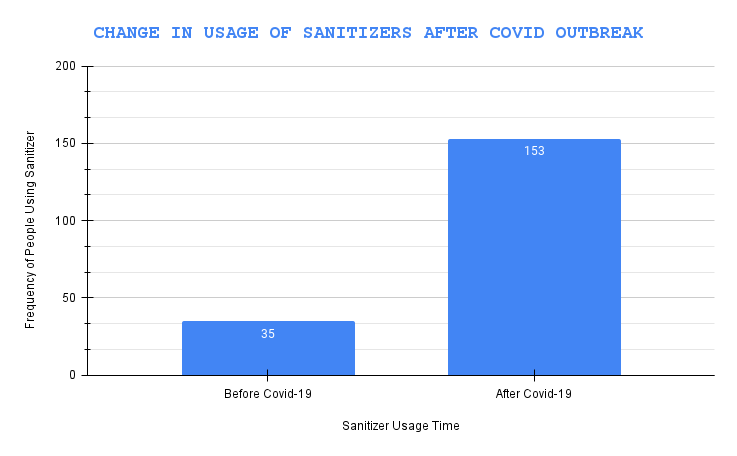
\includegraphics[width=0.8\linewidth]{IMAGES/Image 36.png}
	\caption{Sanitizer Usage}
	\label{G36}
\end{figure}

\ 

In the Bar diagram \ref{G36} represents the results of the above-mentioned survey, categorized by the Pre-COVID and Post-COVID usage of Sanitizers  

The diagram illustrates a significant change in the frequency of sanitizer usage time before and after COVID-19. Before the pandemic, the frequency of people using sanitizer was $35$, whereas after COVID-19, this frequency increased substantially to $153$. This considerable uptick in sanitizer usage suggests a heightened awareness and adherence to hygiene practices post-COVID-19. 

\

The substantial increase in frequency may be indicative of a broader societal shift towards prioritizing preventive measures for health and safety in response to the pandemic.

\section{Financial Coping Skills}

\begin{figure}[h!]
	\centering
	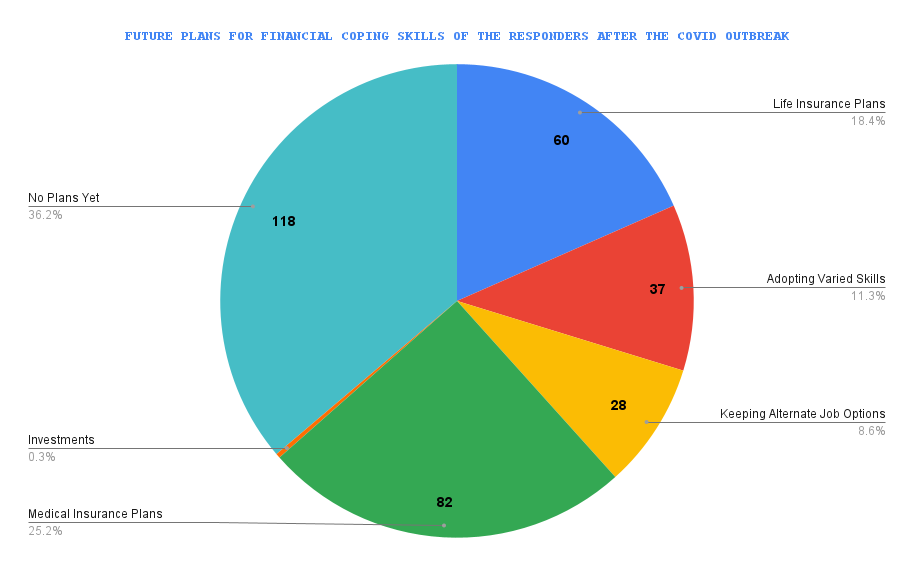
\includegraphics[width=0.9\linewidth]{IMAGES/Image 37.png}
	\caption{Financial Coping Skills}
	\label{G37}
\end{figure}

\ 

The Pie chart in \ref{G37} represents the distribution of Post-COVID financial coping strategies, with notable emphasis on medical insurance, varied skill acquisition, and a substantial portion undecided about future plans.

\

In summary, the analysis of post-COVID financial coping plans, as depicted in the chart, reveals a diverse landscape. Notably, $25.2\%$ of respondents prioritize their well-being with medical insurance, while $18.4\%$ consider life insurance. A proactive approach is evident, with $11.3\%$ aiming to acquire diverse skills, and $8.6\%$ exploring alternate job options. Surprisingly, only $0.3\%$ express plans for investments. Significantly, $36.2\%$ of individuals have yet to formalize specific financial strategies, underscoring the prevailing uncertainty. 

\

This numerical breakdown emphasizes the variety of approaches, highlighting the intricate and individualized nature of post-pandemic financial planning among surveyed individuals.

\section{General awareness in controlling a pandemic in near-future}

\begin{figure}[h!]
	\centering
	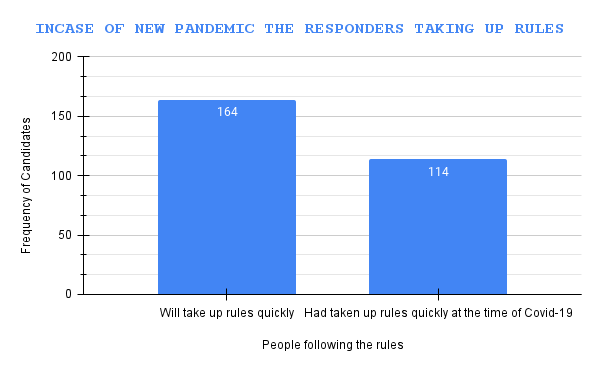
\includegraphics[width=0.9\linewidth]{IMAGES/Image 38.png}
	\caption{General awareness of public}
	\label{G38}
\end{figure}

\ 

As we can see from Figure \ref{G38} the harsh matter of fact, it is likely for the world to face more pandemics in the near future, followed by COVID-19. However a word of hope is that we have, from our data set, the number of people likely to follow government prescribed guidelines has increased quite a bit compared to that at the time of onset of COVID-19.

\

Out of $230$ individuals, the number $114$ of people, taking up guidelines and rules at the time of the Corona Outbreak is quite less than the number $164$ of people willing to quickly follow the new guidelines if a similar history of COVID repeats itself in near future. 

\

It is conclusive that a general awareness regarding the pandemic and its control have grown among the responders.

\chapter{Estimation}
\section{Analysis on Weight Difference before and after COVID-situation}

Here our goal is to check if COVID-situation had any impact on weight. We collected data from 230 individuals and we have done the following study depending on that data.

\ 

Consider $(X_{1}, Y_{1})$, .... , $(X_{n}, Y_{n})$ being paired data of $n$-individuals, where

$$X_{1}, .. , X_{n} \ \sim \ \text{IID} \ N(\mu, \sigma^{2}) \ : \ \text{represents weight distribution of $n$-individuals before COVID}$$
$$Y_{1}, .. , Y_{n} \ \sim \ \text{IID} \ N(\mu, \sigma^{2}) \ : \ \text{represents weight distribution of $n$-individuals after COVID}$$

\ 

Here, 
$$E(X_{i}) \ = \ \mu_{1} , \ V(X_{i}) \ = \ \sigma_{1}^{2} , \ \forall \ i \ = \ 1, 2, ... , n$$
$$E(Y_{i}) \ = \ \mu_{2} , \ V(Y_{i}) \ = \ \sigma_{2}^{2} , \ \forall \ i \ = \ 1, 2, ... , n$$
where $\sigma_{1}, \sigma_{2}$ are unknown.

\ 

Assuming normality, we will check if weight remains same before and after COVID against alternative hypothesis or it does not.

\ 

\textbf{Hypothesis}:
$$H_{0} \ : \ \mu_{1} \ = \ \mu_{2} \ \text{vs} \ H_{1} \ : \ \mu_{1} \ \neq \ \mu_{2}$$

\ 

Here, $(X_{i}, Y_{i}) \ \sim \ \text{BVN} \ (\mu_{1}, \ \mu_{2}, \ \sigma_{1}^{2}, \ \sigma_{2}^{2}, \ \rho)$, where $\rho$ being the correlation coefficient of $X_{i}$ and $Y_{i}$.

\ 

Take, 
$$D_{i} \ = \ X_{i} \ - \ Y_{i}, \ \forall \ i \ = \ 1, 2, ... , n$$
$$D_{1}, ..., D_{n} \ \text{are IID} \ N(\mu_{1}, \ \mu_{2}, \ \sigma^{2}), \ \sigma^{2} \ \text{unknown}.$$
where,
$$\sigma^{2} \ = \ V(X) \ + \ V(Y) \ - \ 2 \text{Cov} (X, Y)$$
$$= \ \sigma_{1}^{2} \ + \ \sigma_{2}^{2} \ - \ 2 \rho \sigma_{1} \sigma_{2}$$

\ 

Now, the above test becomes equivalent to one sample test
$$H_{0} \ : \ \mu \ = \ 0 \ \text{vs} \ H_{1} \ : \ \mu \ \neq \ 0 \ \text{with unknown} \ \sigma^{2}$$
where, $\mu \ = \ \mu_{1} \ - \ \mu_{2}$.

\

 In this two-tailed test, consider
 $$\Bar{D} \ = \ \frac{D_{1} \ + ..... + \ D_{n}}{n}$$
 $$E[\Bar{D}] \ = \ E[\frac{D_{1} \ + ..... + \ D_{n}}{n}] \ = \ \frac{n\mu}{n} \ = \ \mu$$
 $$V[\Bar{D}] \ = \ V[\frac{D_{1} \ + ..... + \ D_{n}}{n}] \ = \ \frac{1}{n^{2}} \{ V[D_{1}] \ + ... + \ V[D_{n}] \}$$
 $$= \ \frac{1}{n^{2}} \ n\sigma^{2} \ = \ \frac{\sigma^{2}}{n}, \ \ \text{as \ $D_{1}, ... , D_{n}$, \ are IID}$$

 \ 

 thus, $\Bar{D} \ \sim \ N(\mu, \ \frac{\sigma^{2}}{n})$.

 \ 

 \textbf{Test Statistics}:
Consider following test-statistic using paired t-test.
$$T \ = \ \frac{\Bar{D} \ - \ \mu}{\frac{s}{\sqrt{n}}} , \ \ \text{where $s$ being sample standard-deviation}$$

and $T \ \sim t_{n-1}$, i.e. $t$-distribution with $(n-1)$ degrees of freedom.

\ 

Now, based on our data collected form $n \ = \ 231$ observations :
$$\text{mean} \ = \ \Bar{d} \ = \ 3.058696$$
$$\text{median} \ = \ m_{e} \ = \ 3$$
$$\text{variance} \ = \ 45.643920$$
$$\text{standard deviation} \ = \ 6.756028$$

\ 

Now, under the null-hypothesis $\mu \ = \ 0$ and $s \ = \ 0$,
$$T \ = \ \frac{\Bar{D} \sqrt{n}}{s}$$

using the above data,
$$t \ \approx \ 6.866079, \ \text{observed value of} \ T.$$

\ 

\textbf{Critical Region}:
Since, $n \ = \ 230$ and d.f. $= \ 229$, then
$$T \ \sim \ t_{229, \ 0.975}$$
thus critical region at $5 \%$ level of significance is
$$(-\infty , \ 1.9709] \ \bigcup \ [1.9709, \ \infty).$$

\ 

\textbf{Decision Rule}: To make our decision, we will check if test-statistics lie in confidence interval or not. Our test-statistic is $t \ = \ 6.866079$.\\
If $t$ lies within critical region, we reject null-hypothesis.

\ 

\textbf{Decision}: Since, 
$$t \ = \ 6.866079 \ > \ t_{229, \ 0.975} \ = \ 1.9709$$
i.e. $t$ lies within the critical region $(-\infty , \ 1.9709] \ \bigcup \ [1.9709, \ \infty)$.\\
Therefore, we reject null hypothesis $H_{0} \ : \ \mu \ = \ 0$ against $H_{1} \ : \ \mu \ \neq \ 0$.

\ 

\textbf{Result Interpretation}: Rejecting null-hypothesis provides strong evidence that there is a statistically significant difference in weights before and after COVID-19.

\ 

Hence, our study shows COVID-19 pandemic might had an impact on individual's weight.

\ 

Below, we provide a pictorial representation of our data set of weight difference :

\ 

\begin{figure}[h!]
	\centering
	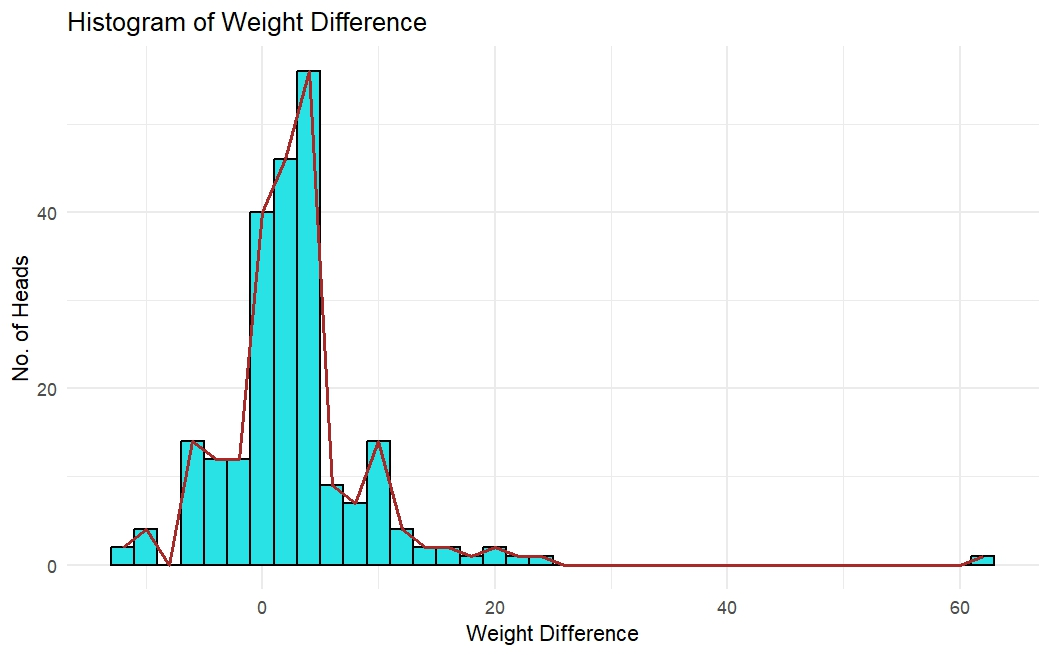
\includegraphics[width=0.7\linewidth]{IMAGES/Image 39.jpg}
	\caption{Difference in Weights}
	\label{G39}
\end{figure}

\ 

We have outliers in our data set. Except these, our data set is clustered between $-20$ to $30$, which indicates persons under study may have encountered significant changes in their weights.

\ 

From the graph above shown (figure \ref{G39}), indicates the mean is greater than zero, which means there is a high probability that individual's had his/her weight decreased after COVID-situation.


\chapter{Hypothesis Testing}
\section{Analysis on Weight Difference before and after COVID outbreak}

\

Here our goal is to check whether the COVID-situation had an impact on weight. We collected data from $230$ individuals and we have done the following study depending on that data.

\ 

Consider $(X_{1}, Y_{1})$, \ldots , $(X_{n}, Y_{n})$ being paired data of $n$-individuals, where :

$$X_{1}, \ldots , X_{n} \ \sim \ \text{IID} \ N(\mu, \sigma^{2}) \ : \ \text{weight distribution of $n$-individuals before COVID}$$
$$Y_{1}, \ldots , Y_{n} \ \sim \ \text{IID} \ N(\mu, \sigma^{2}) \ : \ \text{weight distribution of $n$-individuals after COVID}$$

Here, 
$$E(X_{i}) \ = \ \mu_{1} , \ V(X_{i}) \ = \ \sigma_{1}^{2} , \ \forall \ i \ = \ 1, 2, \ \ldots \ , n$$
$$E(Y_{i}) \ = \ \mu_{2} , \ V(Y_{i}) \ = \ \sigma_{2}^{2} , \ \forall \ i \ = \ 1, 2, \ \ldots \ , n$$
where $\sigma_{1}, \sigma_{2}$ are unknowns.

\ 

Assuming normality, we will assess whether the weights remain the same before and after COVID, testing against the alternative hypothesis that they do not.

\ 

\textbf{Hypothesis}:
$$H_{0} \ : \ \mu_{1} \ = \ \mu_{2} \ \text{  vs  } \ H_{1} \ : \ \mu_{1} \ \neq \ \mu_{2}$$

\ 

Here, $(X_{i}, Y_{i}) \ \sim \ \text{BVN} \ (\mu_{1}, \ \mu_{2}, \ \sigma_{1}^{2}, \ \sigma_{2}^{2}, \ \rho)$, where $\rho$ being the correlation coefficient of $X_{i}$ and $Y_{i}$.

\ 

So Let's take, 
$$D_{i} \ = \ X_{i} \ - \ Y_{i}, \ \forall \ i \ = \ 1, 2, ... \ , n$$
$$D_{1}, \ \ldots \ , D_{n} \ \text{are IID} \ N(\mu_{1} - \mu_{2}, \ \sigma^{2}), \text{ where } \ \sigma^{2} \ \text{unknown}.$$

\newpage

where we have,
$$\sigma^{2} \ = \ V(X) \ + \ V(Y) \ - \ 2 \cdot \text{Cov} (X, Y)$$
$$= \ \sigma_{1}^{2} \ + \ \sigma_{2}^{2} \ - \ 2 \cdot \rho \cdot \sigma_{1} \cdot \sigma_{2}$$

\ 

Now, the above test becomes equivalent to one sample test of
$$H_{0} \ : \ \mu \ = \ 0 \ \text{  vs  } \ H_{1} \ : \ \mu \ \neq \ 0 \ \text{with unknown} \ \sigma^{2}$$
where, \ $\mu \ = \ \mu_{1} \ - \ \mu_{2}$.

\

 In this two-tailed test, consider
 $$\Bar{D} \ = \ \frac{D_{1} \ + \ \ldots \ + \ D_{n}}{n}$$
 \[E\left[\Bar{D}\right] = E\left[\frac{D_{1} + \ldots + D_{n}}{n}\right] = \frac{n\cdot\mu}{n} = \mu\]
 \[V\left[\Bar{D}\right] = V\left[\frac{D_{1} + \ldots + D_{n}}{n}\right] = \frac{1}{n^{2}} \left\{ V[D_{1}] + \ldots + V[D_{n}] \right\}\]
 \[= \frac{1}{n^{2}} \ n\sigma^{2} = \frac{\sigma^{2}}{n}, \quad \text{as $D_{1}, \ \ldots \ , D_{n}$ are IID}\]

 \ 

thus, $\Bar{D} \sim N(\mu, \frac{\sigma^{2}}{n})$.

 \ 

\textbf{Test Statistics}:
Consider following test-statistic using paired \textit{$t-test$}.
$$T \ = \ \frac{\Bar{D} \ - \ \mu}{\frac{s}{\sqrt{n}}} , \ \ \text{where $s$ being sample standard-deviation}$$

and $T \ \sim \ t_{n-1}$, i.e. $t$-distribution with $(n-1)$ degrees of freedom.

\ 

Now, based on our data collected form $n \ = \ 230$ observations : 
\begin{center}
    \fbox{\parbox{\textwidth}{
$$\text{Sample Mean} \ = \ \Bar{d} \ = \ 3.058696$$
$$\text{Sample Median} \ = \ m_{e} \ = \ 3$$
$$\text{Sample Variance} \ = \ 45.643920$$
$$\text{Sample Standard deviation} \ = \ 6.756028$$
}}
\end{center}


\newpage 

Now, under the null-hypothesis $\mu \ = \ 0$ and $s \ = \ 0$,
$$T \ = \ \frac{\Bar{D} \cdot \sqrt{n}}{s}$$

using the above data,
$$t \ \approx \ 6.866079, \ \text{observed value of} \ T.$$

\ 

\textbf{Critical Region} :
Since, $n \ = \ 230$ and $d.f.$ \ $= \ 229$, then
$$T \ \sim \ t_{229, \ 0.975}$$
thus critical region at $5\%$ level of significance is
$$(-\infty , \ 1.9709] \ \bigcup \ [1.9709, \ \infty).$$

\ 

\textbf{Decision Rule}: To make our decision, we will check if test-statistics lies in confidence interval or not. Our test-statistic is $t \ = \ 6.866079$.

\

If $t$ lies within the critical region, we reject null-hypothesis.

\ 

\textbf{Decision}: Since, 
$$t \ = \ 6.866079 \ > \ t_{229, \ 0.975} \ = \ 1.9709$$
i.e. $t$ lies within the critical region $(-\infty , \ 1.9709] \ \cup \ [1.9709, \ \infty)$. 

\

Therefore, we \textbf{reject null hypothesis} $H_{0} \ : \ \mu \ = \ 0$ against $H_{1} \ : \ \mu \ \neq \ 0$.

\begin{figure}[h!]
	\centering
	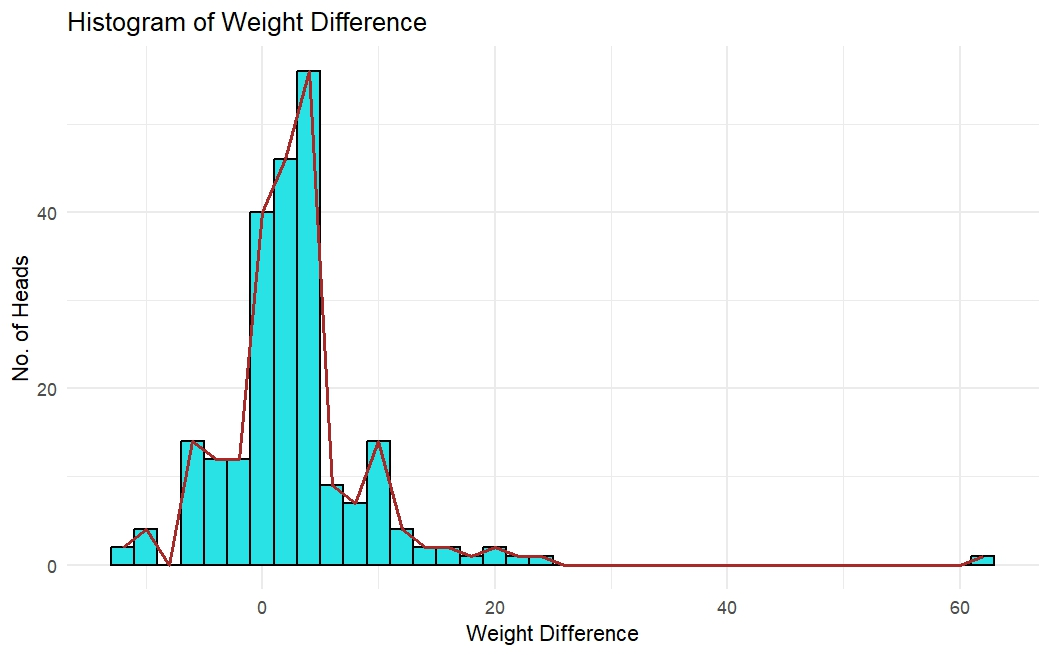
\includegraphics[width=0.7\linewidth]{IMAGES/Image 39.jpg}
	\caption{Difference in Weights}
	\label{G39}
\end{figure}

Above, in Figure \ref{G39} we provide a pictorial representation of our data set of weight difference

\

\textbf{Result Interpretation}: Rejecting null-hypothesis provides strong evidence that there is a statistically significant difference in weights before and after COVID-19.

\ 

Hence, our study shows COVID-19 pandemic might had an impact on individual's weight.
 
\ 

We have outliers in our data set. Except these, our data set is clustered between $-20$ to $30$, which indicates persons under study may have encountered significant changes in their weights.

\ 

From the graph above shown (figure \ref{G39}), indicates the mean is greater than zero, which means there is a high probability that individual's had his/her weight decreased after COVID-situation.


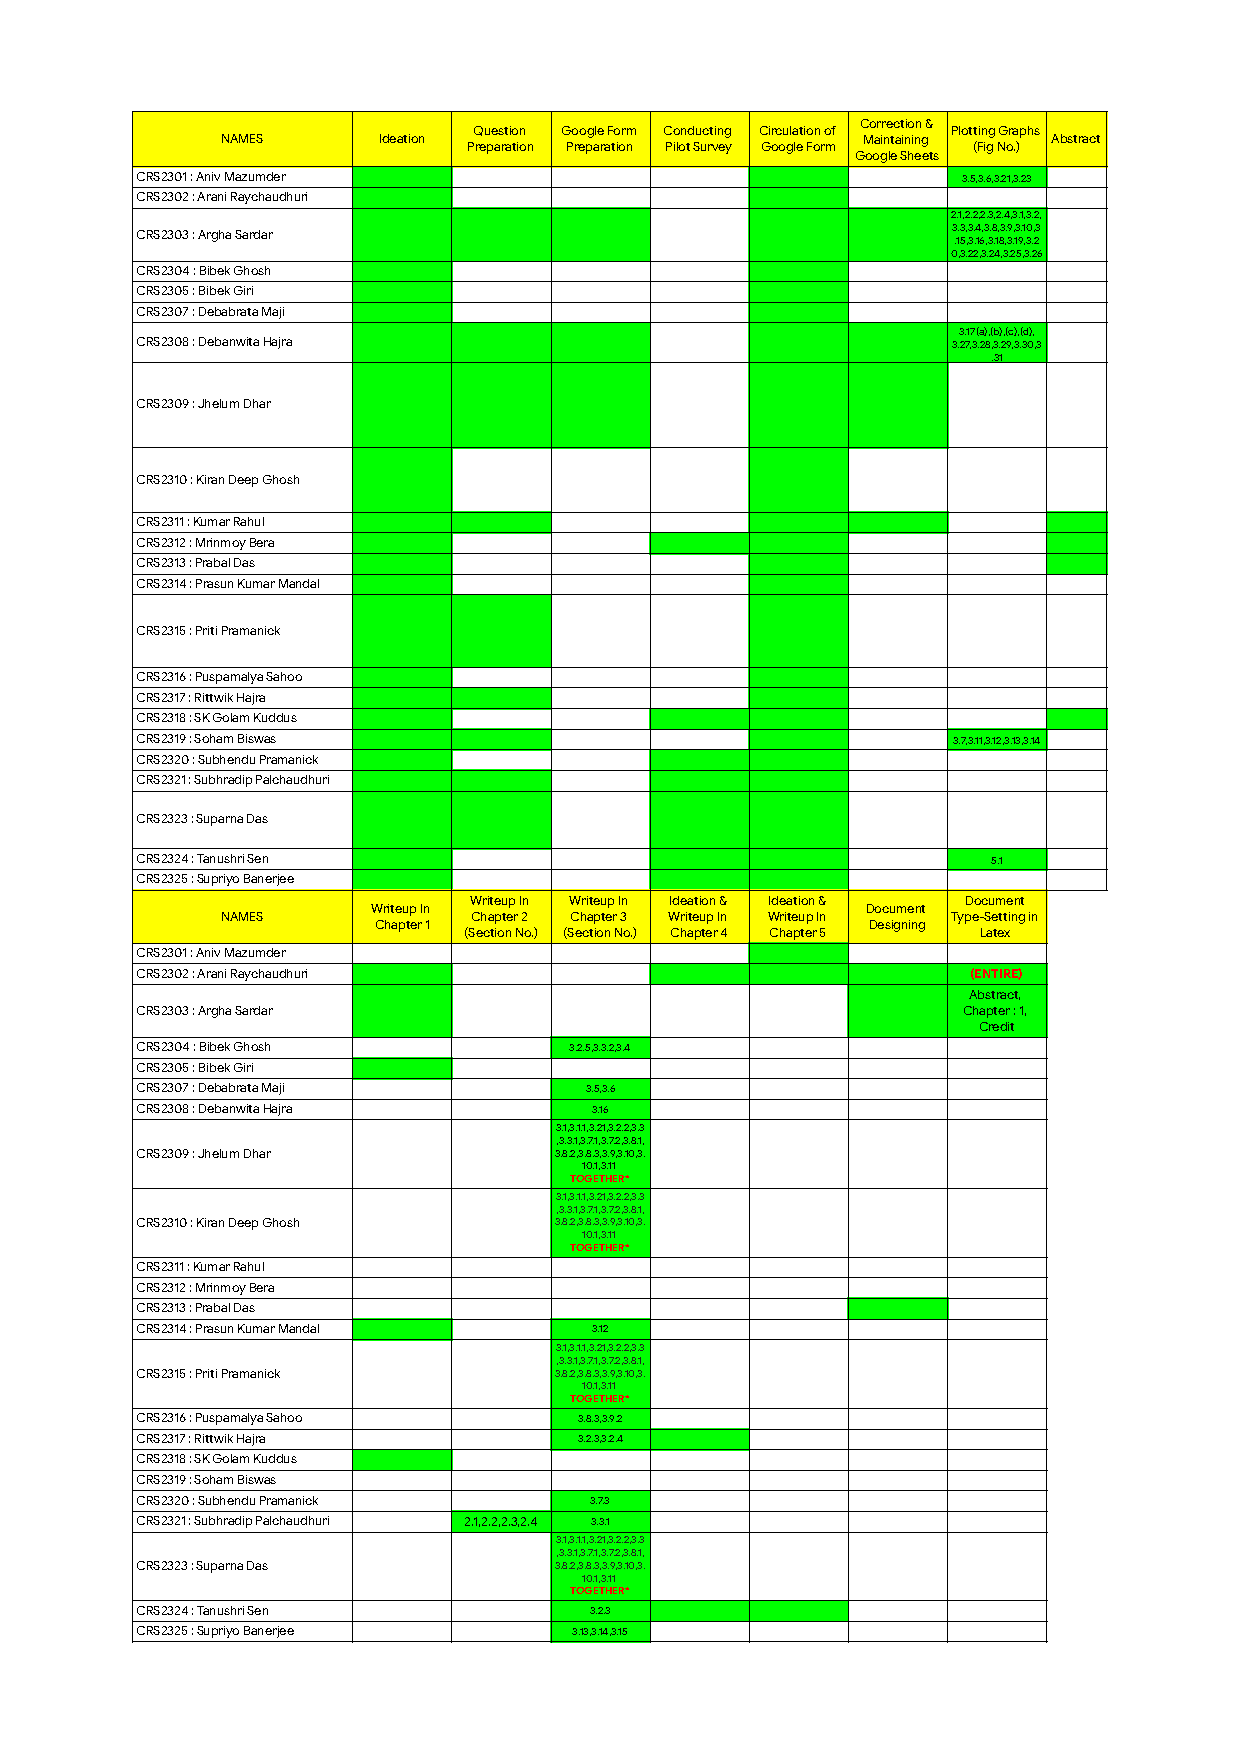
\includepdf[pages=-]{CREDIT.pdf}

\chapter*{Credits}
\addcontentsline{toc}{chapter}{Credits}
\thispagestyle{empty}

\begin{multicols}{2} % Start two-column layout
\begin{itemize}
  \item Aniv Mazumder 
  \item Arani Raychaudhuri 
  \item Argha Sardar
  \item Bibek Ghosh
  \item Bibek Giri
  \item Debabrata Maji 
  \item Debanwita Hajra
  \item Jhelum Dhar
  \item Kiran Deep Ghosh
  \item Kumar Rahul
  \item Mrinmoy Bera
  \item Prabal Das
  \item Prasun Kumar Mandal 
  \item Priti Pramanick
  \item Puspamalya Sahoo 
  \item Rittwik Hajra
  \item SK Golam Kuddus
  \item Soham Biswas
  \item Subhendu Pramanick
  \item Subhradip Palchaudhuri 
  \item Suparna Das
  \item Tanushri Sen
  \item Supriyo Banerjee
\end{itemize}
\end{multicols}

\begin{figure}[h!]
	\begin{subfigure}{0.5\textwidth}
		\centering
		
\includegraphics[width=0.63\linewidth]{IMAGES/FORM.png}
		\caption*{\centering Google Form}
	\end{subfigure}%
	\begin{subfigure}{0.5\textwidth}
		\centering
		
\includegraphics[width=0.63\linewidth]{IMAGES/RESPONSE.png}
		\caption*{\centering Response Sheet}
	\end{subfigure}
	\caption*{\centering PLEASE SCAN THE QR CODES FOR VIEWING THE DOCUMENTS}
\end{figure}


\end{document}